\documentclass[11pt,a4paper]{article}
\usepackage[margin=12mm]{geometry}
\usepackage{amsmath,graphicx}
\graphicspath{{./}}
\title{\textbf{The fit against every set in it}\\[2mm]
\large run \texttt{C1\_with\_compass}, 11 sets, 1555 points,
$\chi^2/\mathrm{ndf}=1.4018$}
\author{}\date{18 September 2026}
\begin{document}\maketitle
\noindent
Data red, model blue.  Each panel carries its own kinematics and $\chi^2$; the
model curve includes the fitted normalisation where the set has one (De Masi
1.0586, Hall A neutron 0.9776, Hall A 2016 1.0583).  Only sets that are
\emph{in} the fit are shown here --- for the blind predictions (CLAS12 cross
sections, the digitised De Masi $\alpha$) see the full report.
\begin{figure}[p]\centering
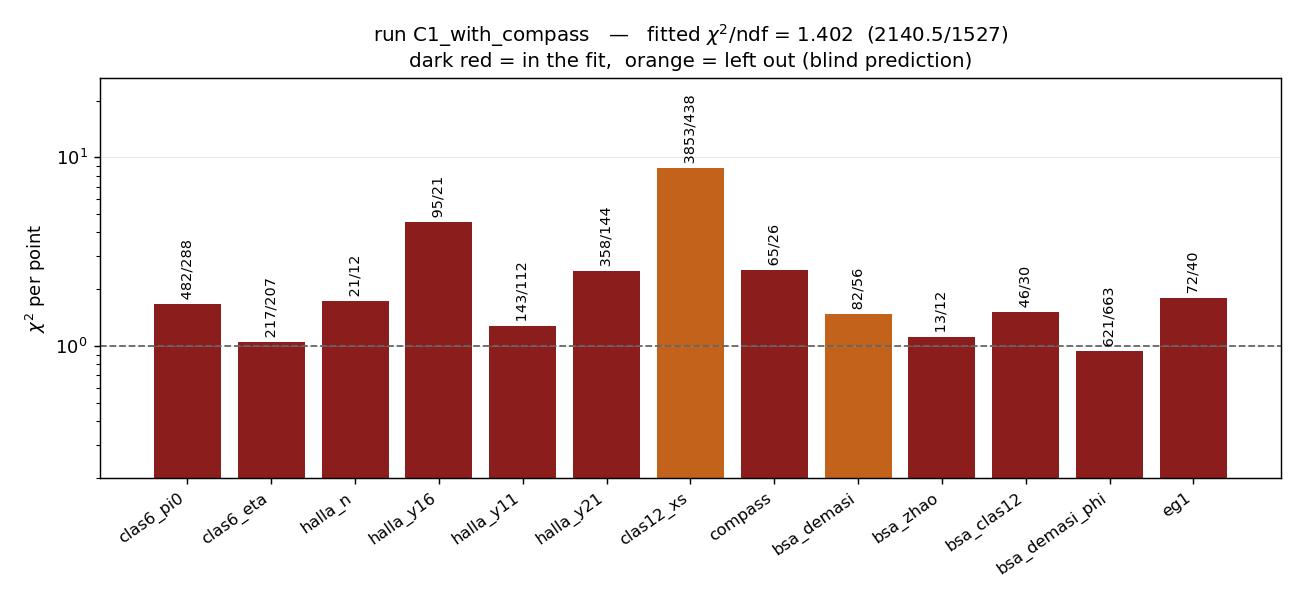
\includegraphics[width=\textwidth]{00_chi2_summary.png}
\caption{All thirteen sets at a glance, fitted and blind.}
\end{figure}
\clearpage
\begin{figure}[p]\centering
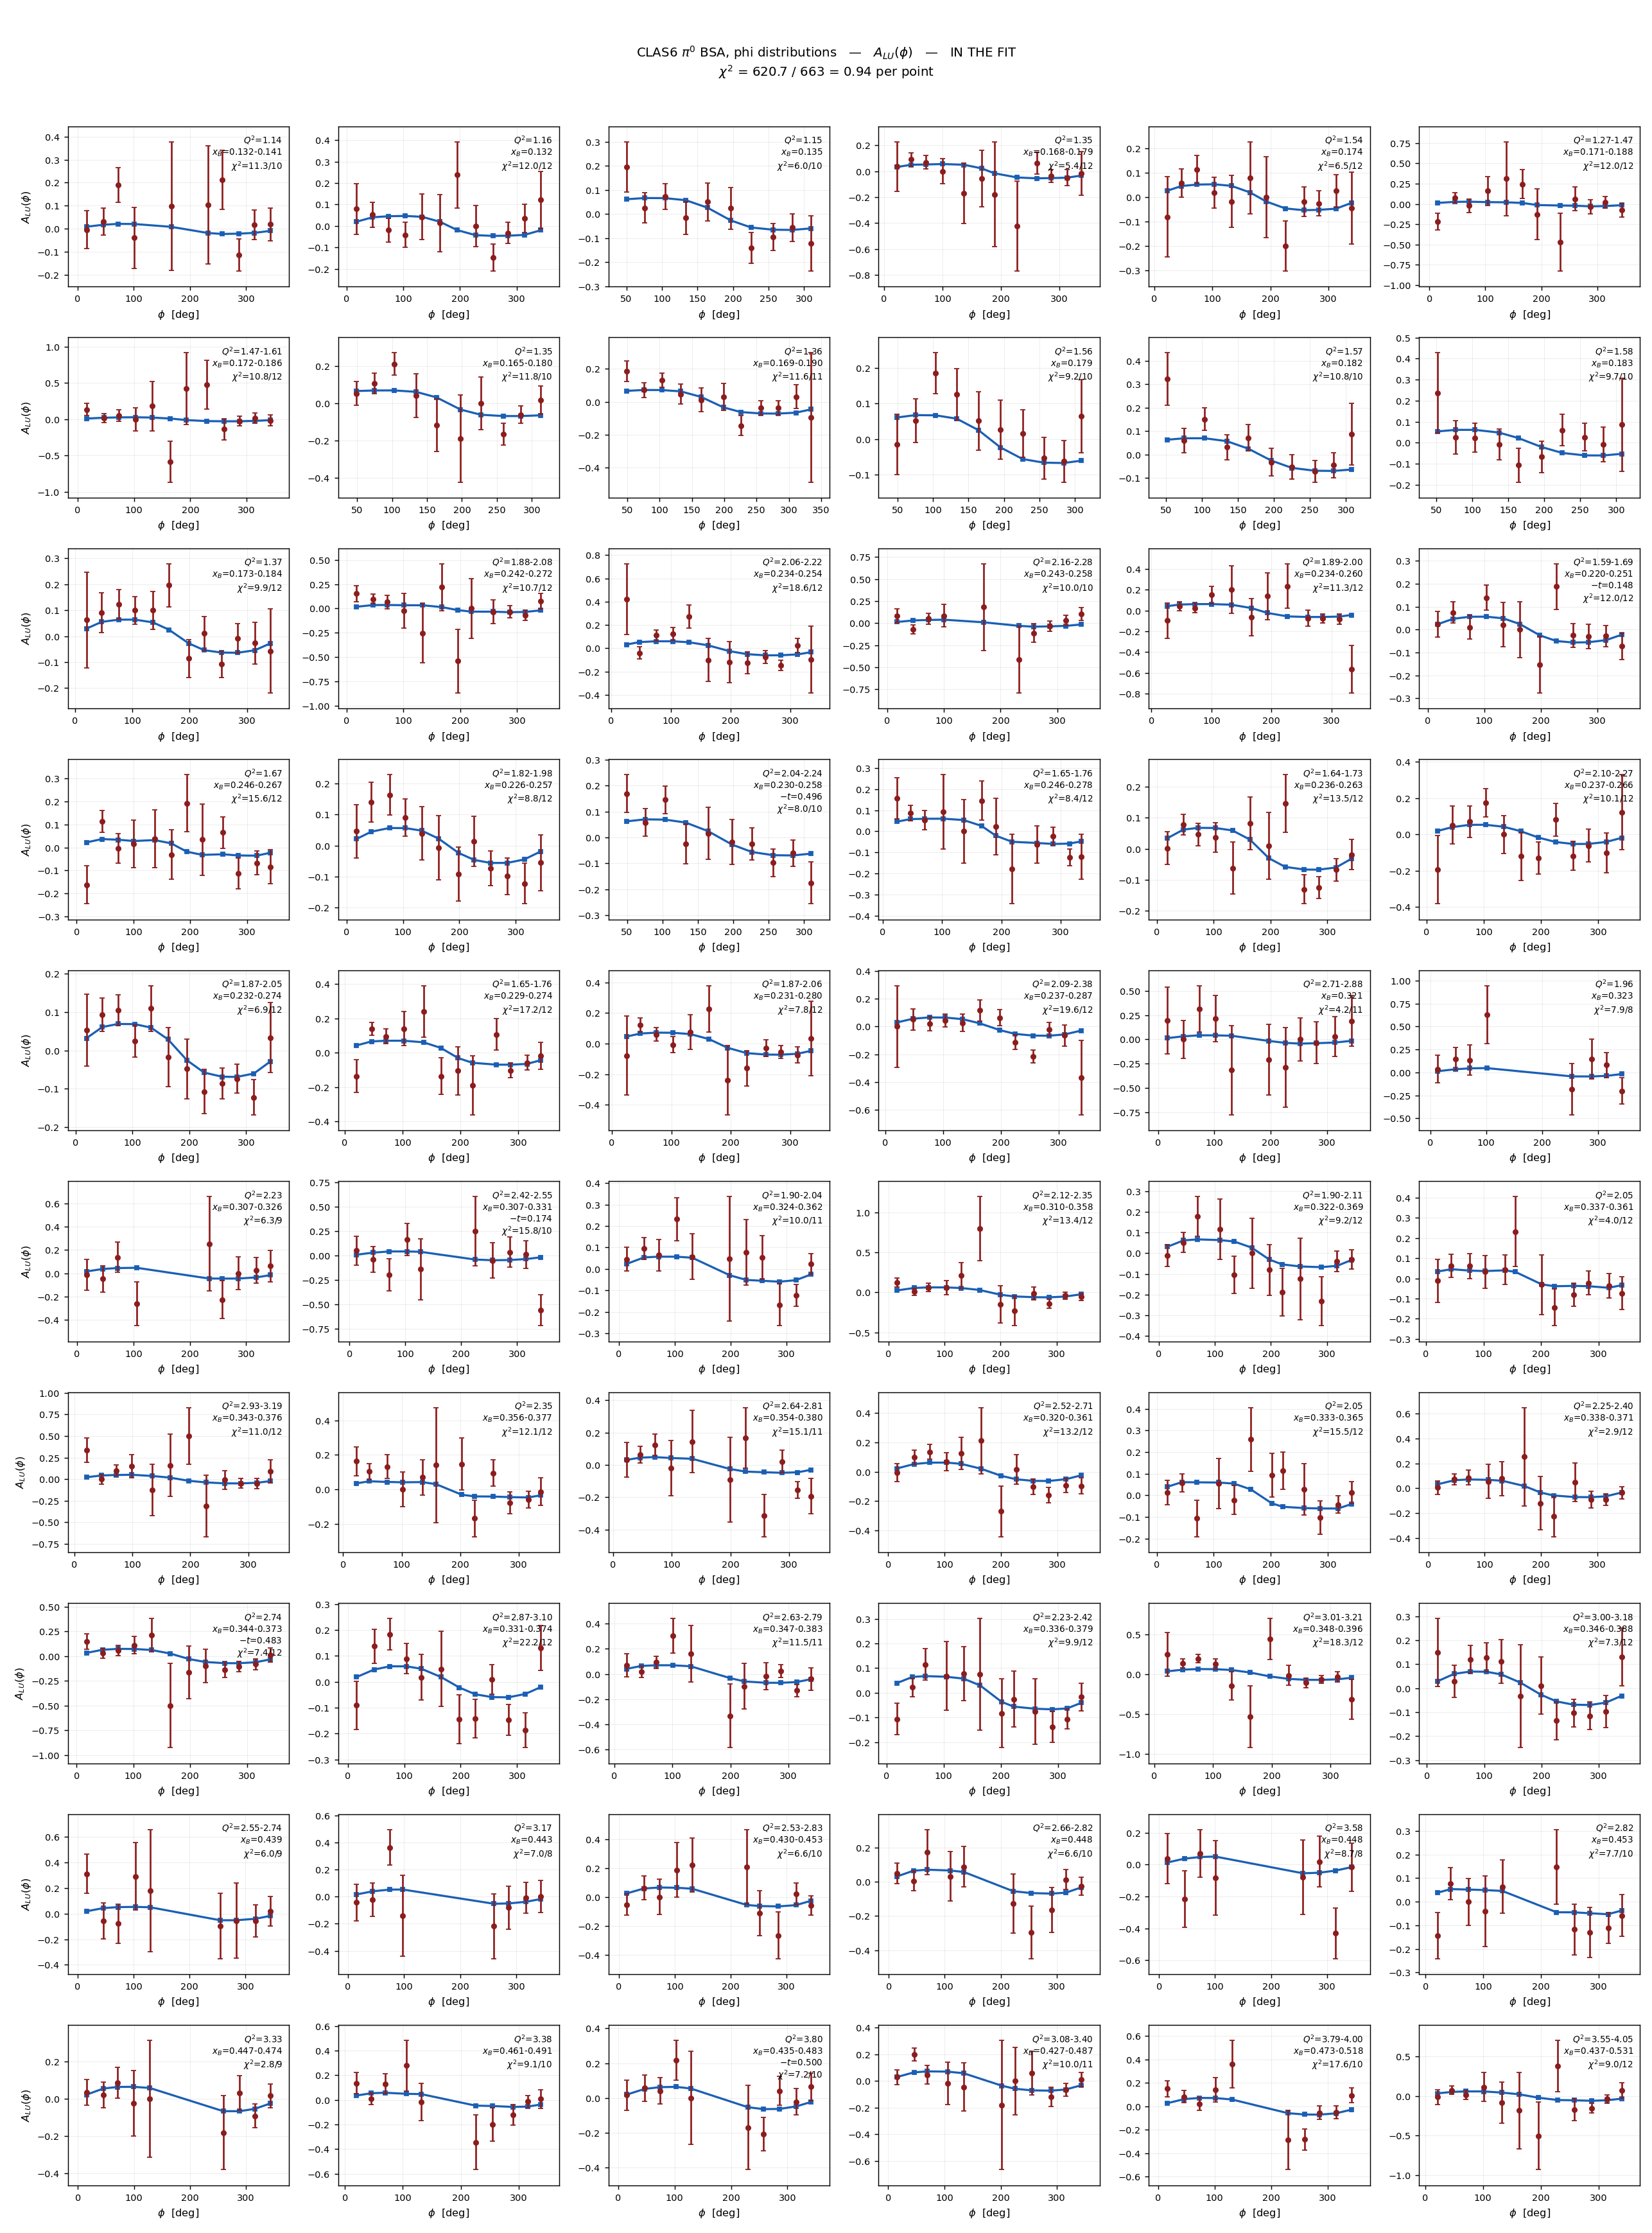
\includegraphics[width=\textwidth]{01_bsa_demasi_phi_in_A_phi.png}
\caption{De Masi, $A_{LU}(\phi)$, all 60 bins --- $A_{LU}(\phi)$.  This set: $\chi^2 = 620.7/663 = 0.94$ per point.}
\end{figure}

\begin{figure}[p]\centering
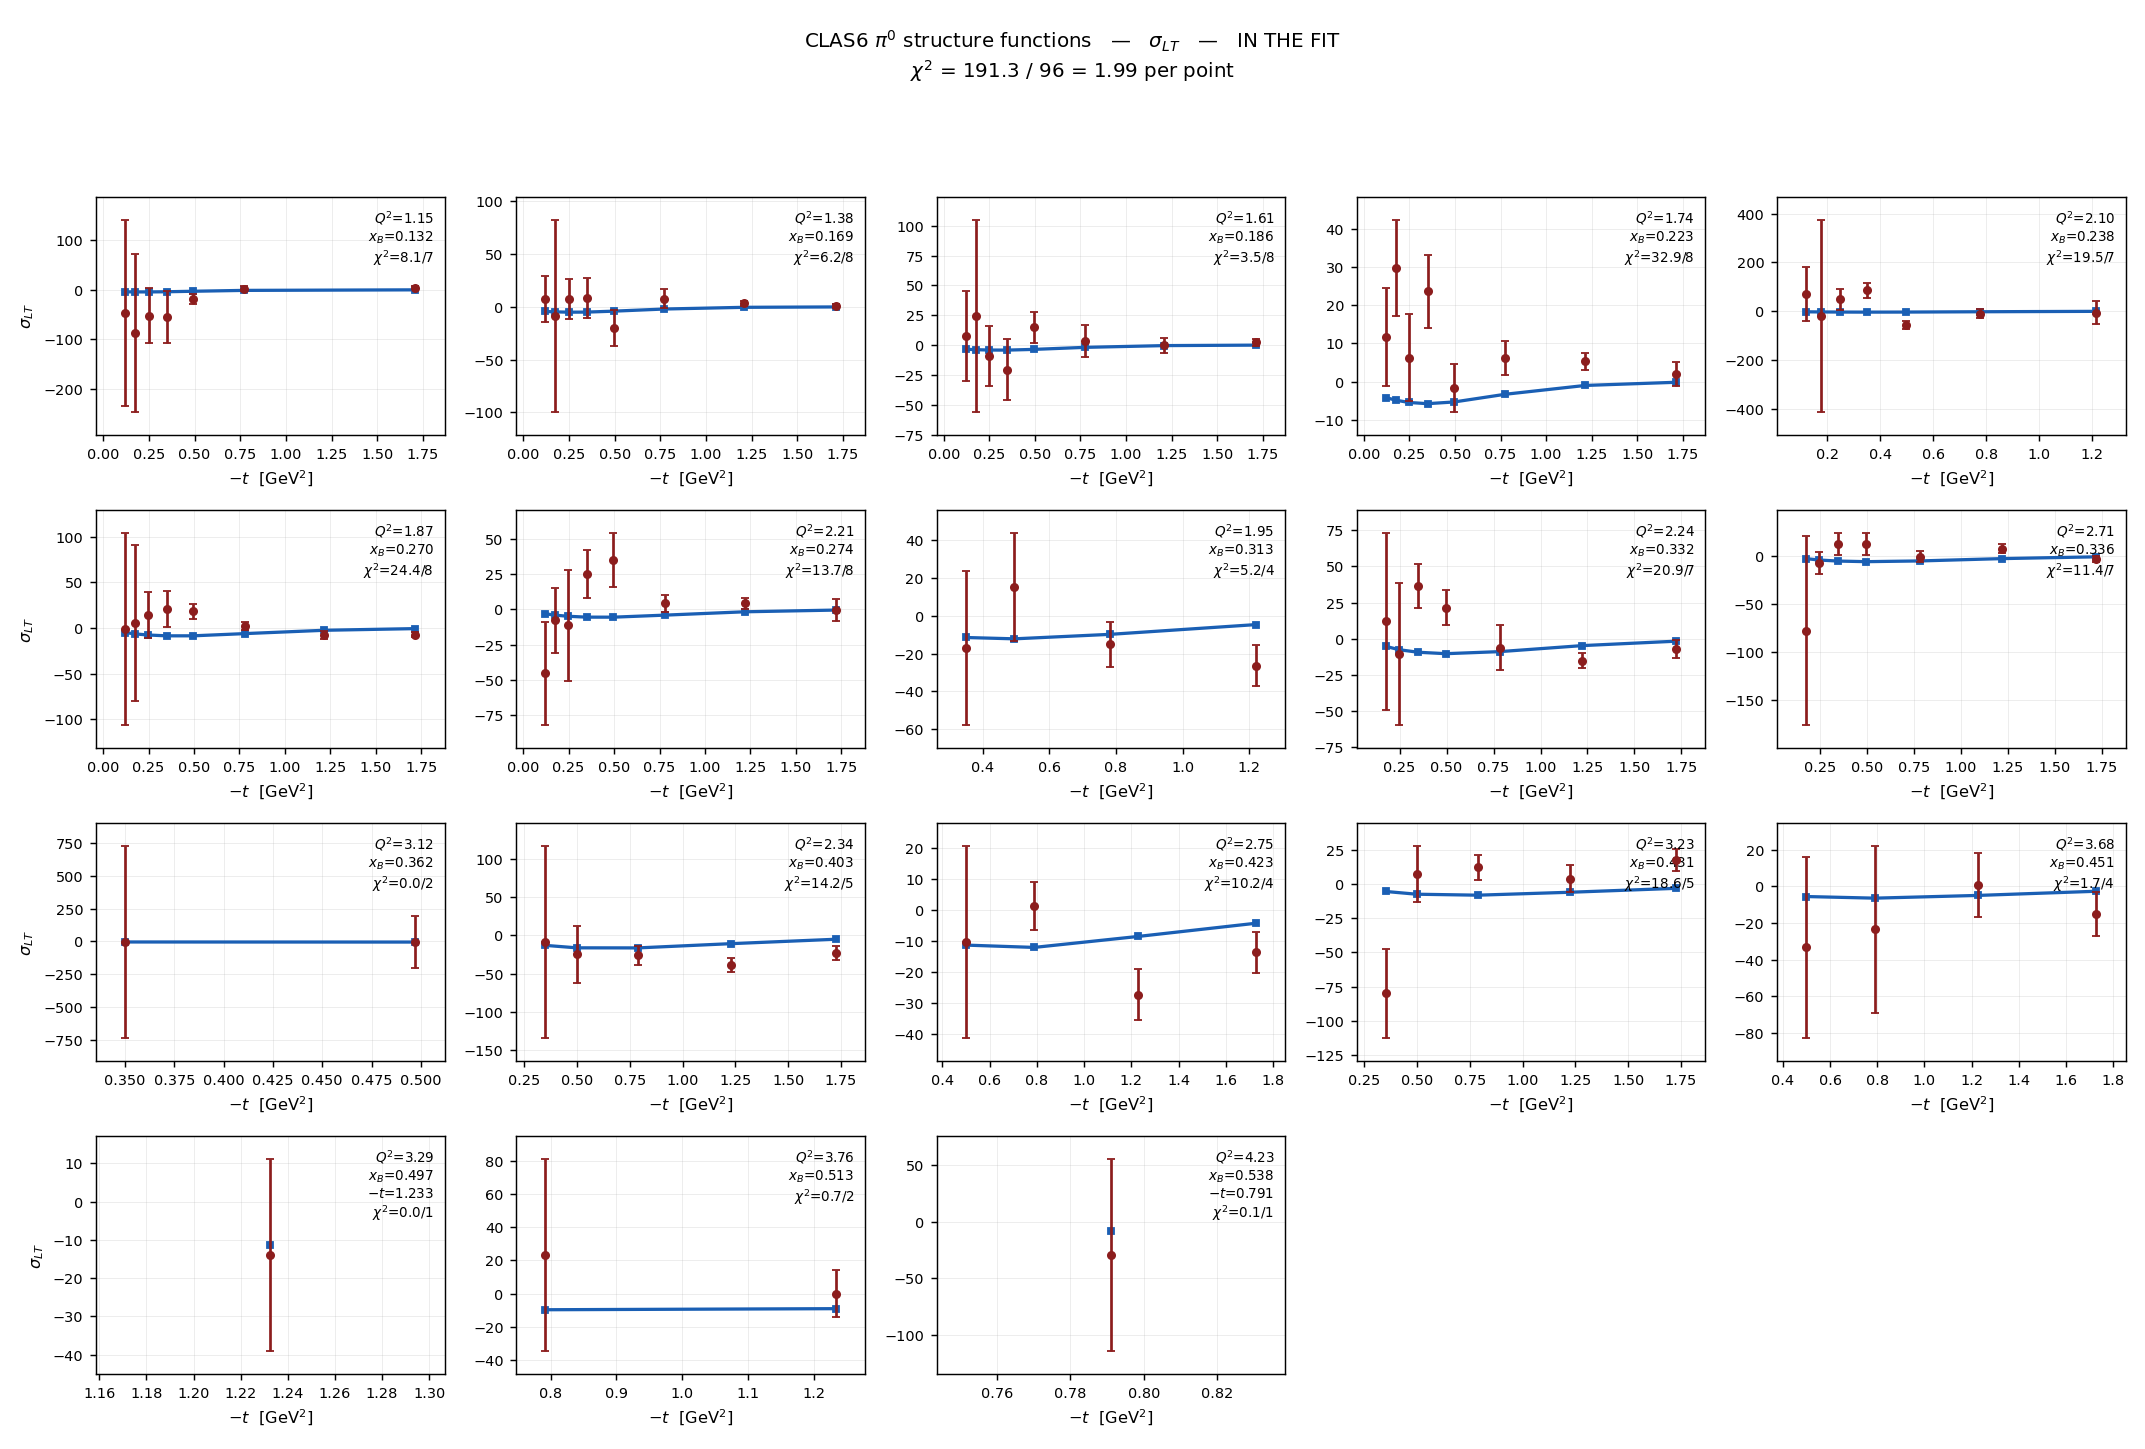
\includegraphics[width=\textwidth]{02_clas6_pi0_in_LT.png}
\caption{CLAS6 $\pi^0$ off the proton --- $\sigma_{LT}$.  This set: $\chi^2 = 482.4/288 = 1.68$ per point.}
\end{figure}

\begin{figure}[p]\centering
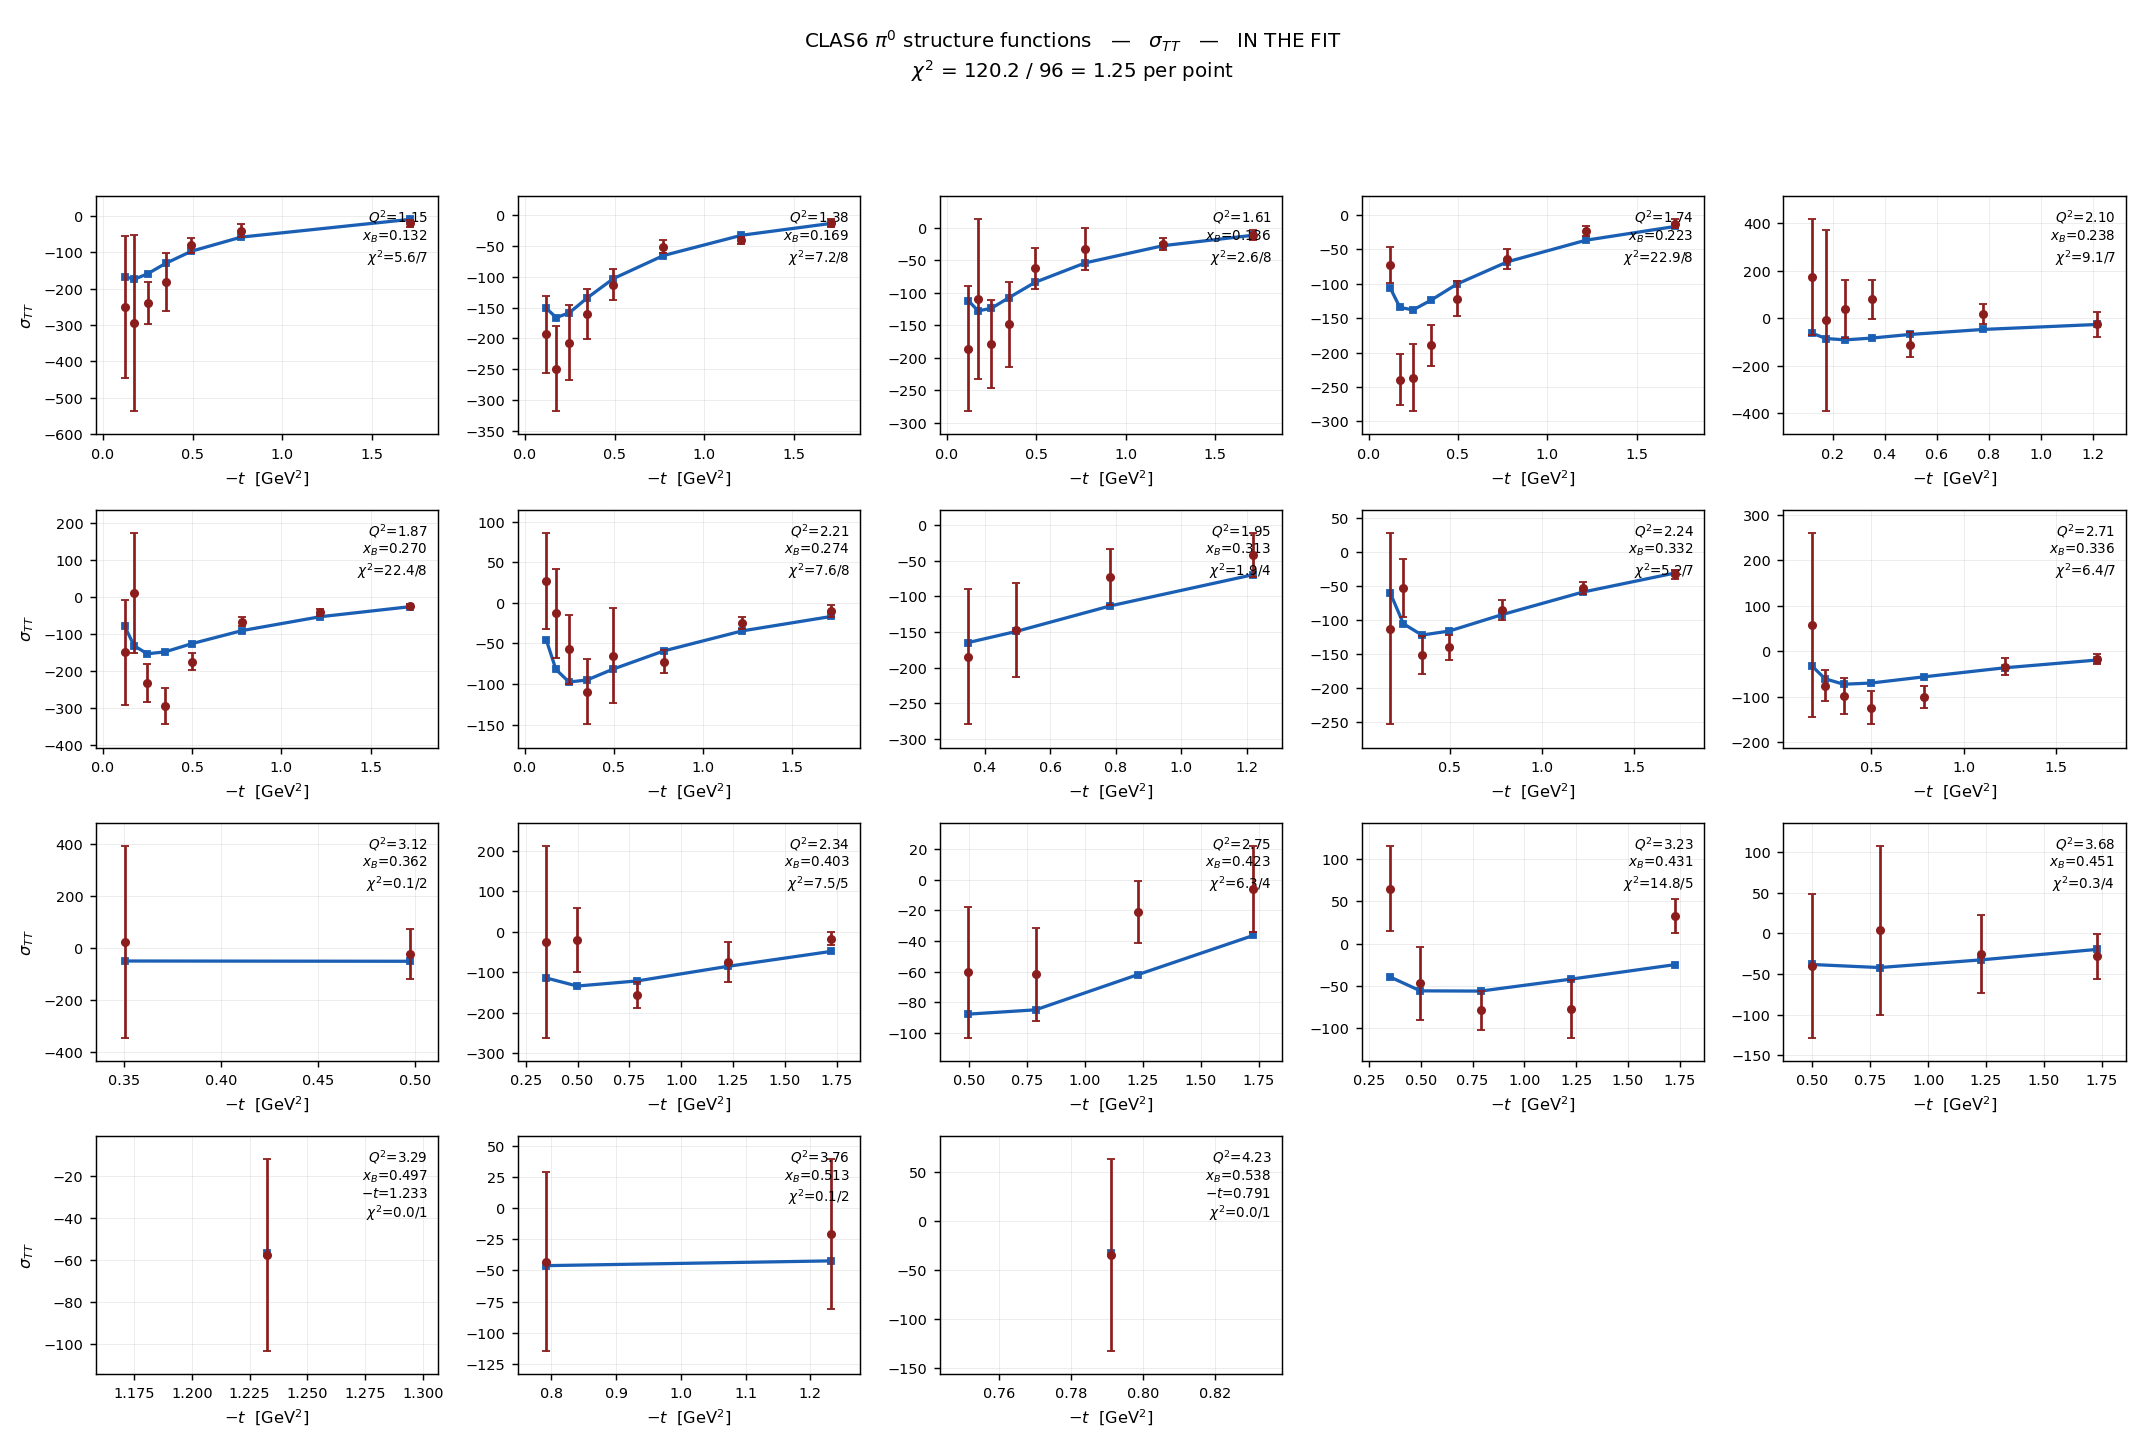
\includegraphics[width=\textwidth]{02_clas6_pi0_in_TT.png}
\caption{CLAS6 $\pi^0$ off the proton --- $\sigma_{TT}$.  This set: $\chi^2 = 482.4/288 = 1.68$ per point.}
\end{figure}

\begin{figure}[p]\centering
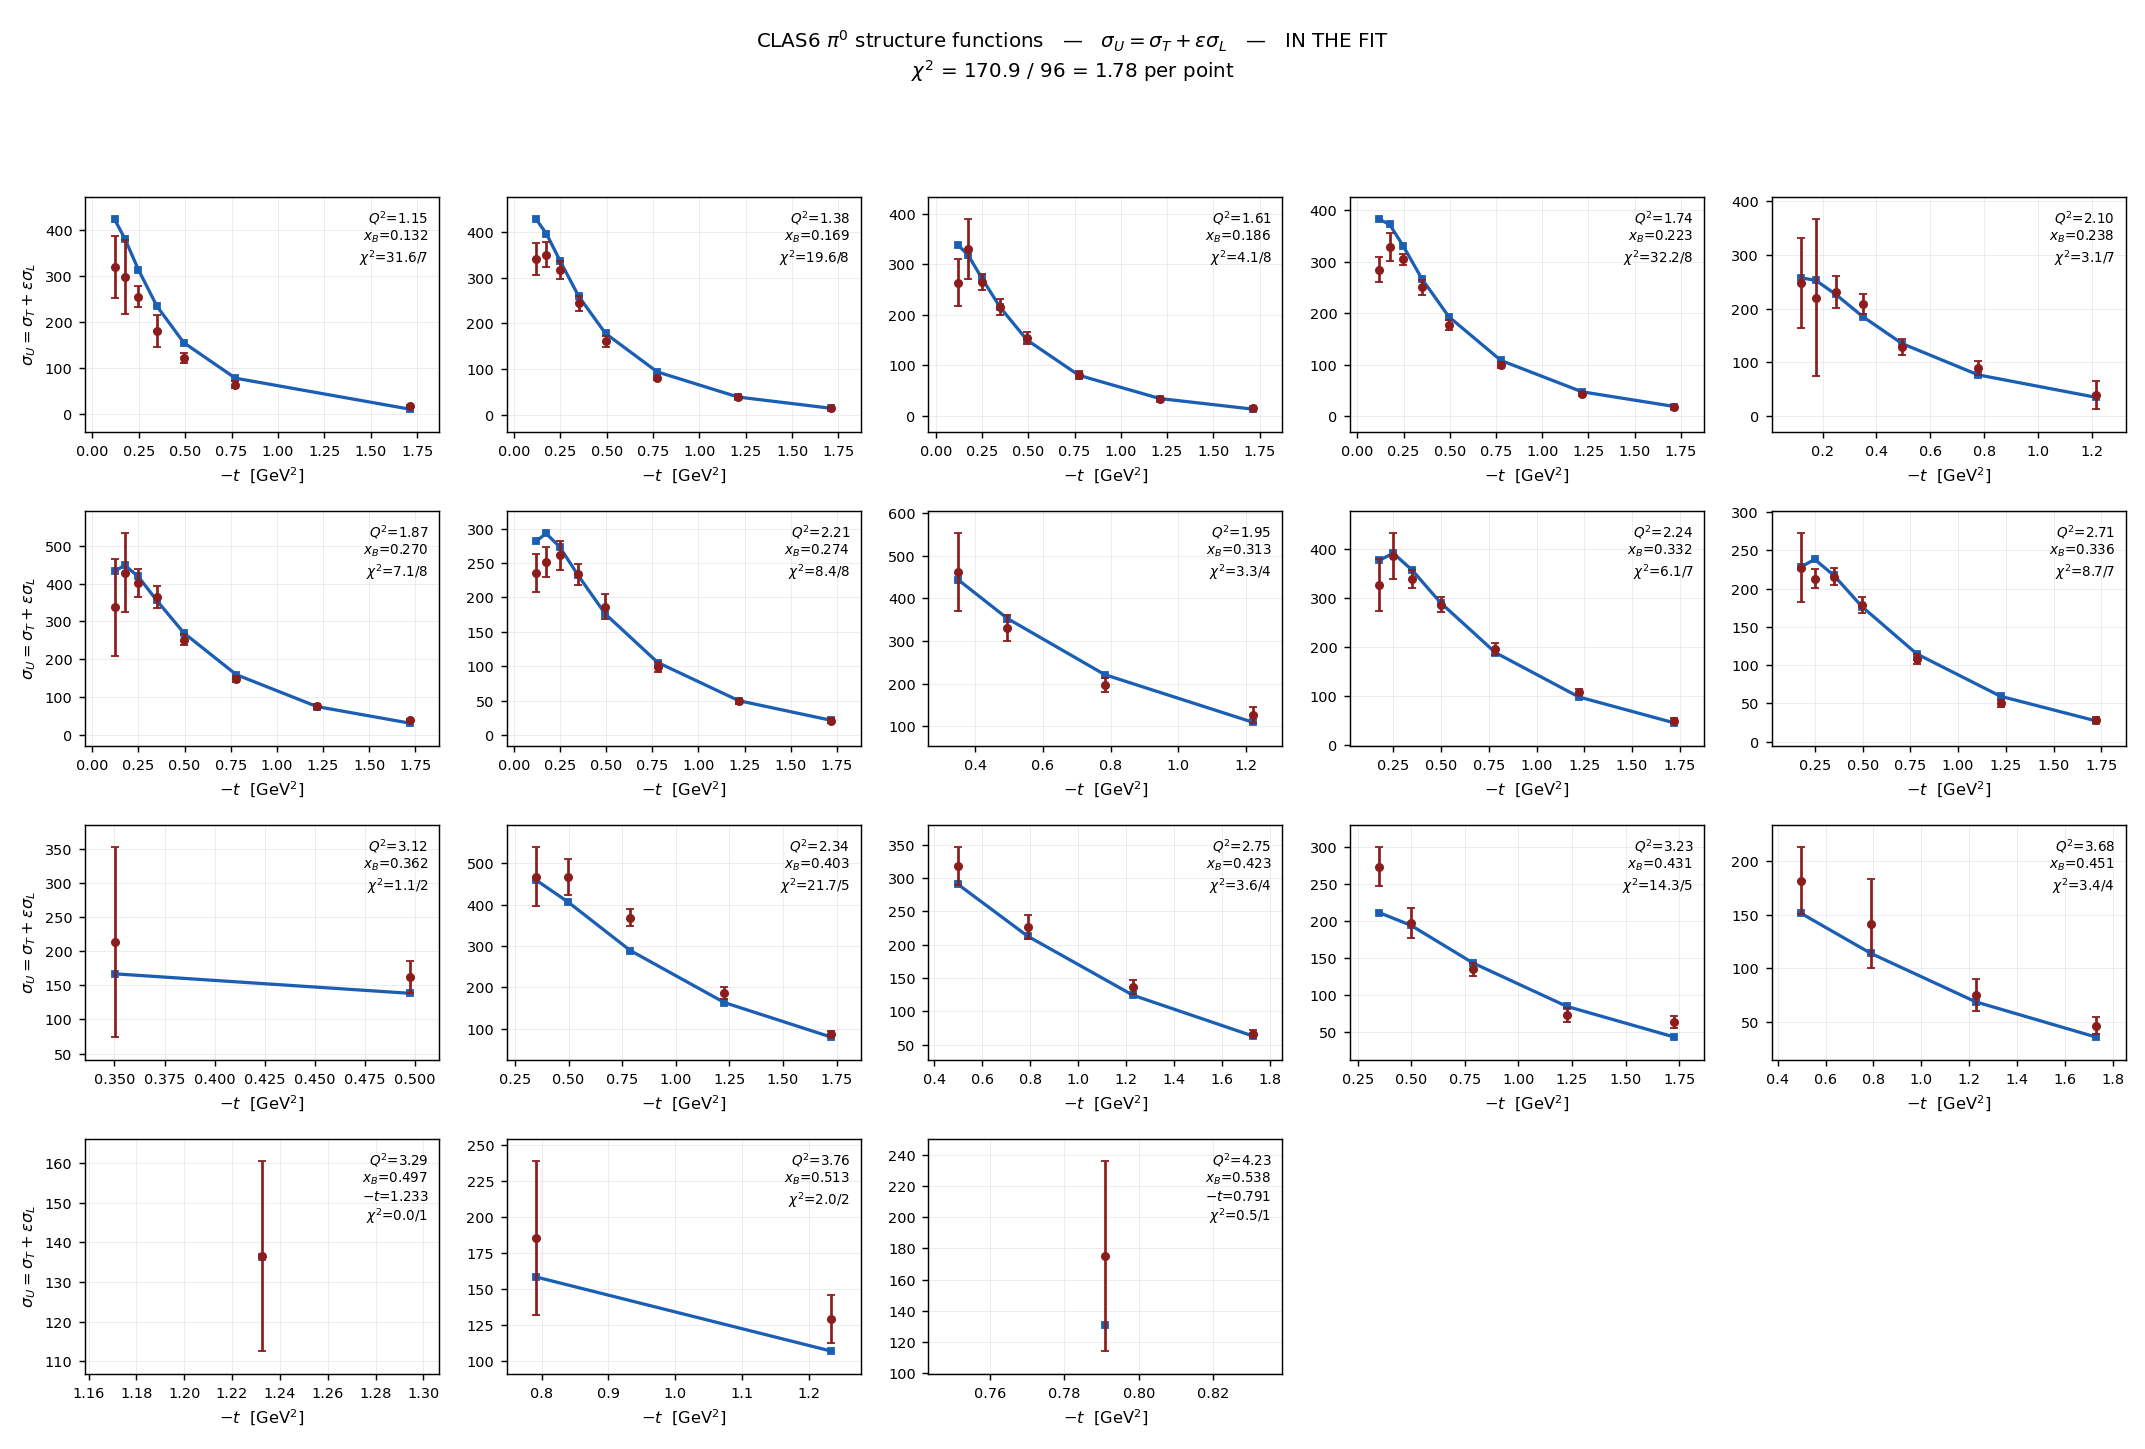
\includegraphics[width=\textwidth]{02_clas6_pi0_in_U.png}
\caption{CLAS6 $\pi^0$ off the proton --- $\sigma_U=\sigma_T+\epsilon\sigma_L$.  This set: $\chi^2 = 482.4/288 = 1.68$ per point.}
\end{figure}

\begin{figure}[p]\centering
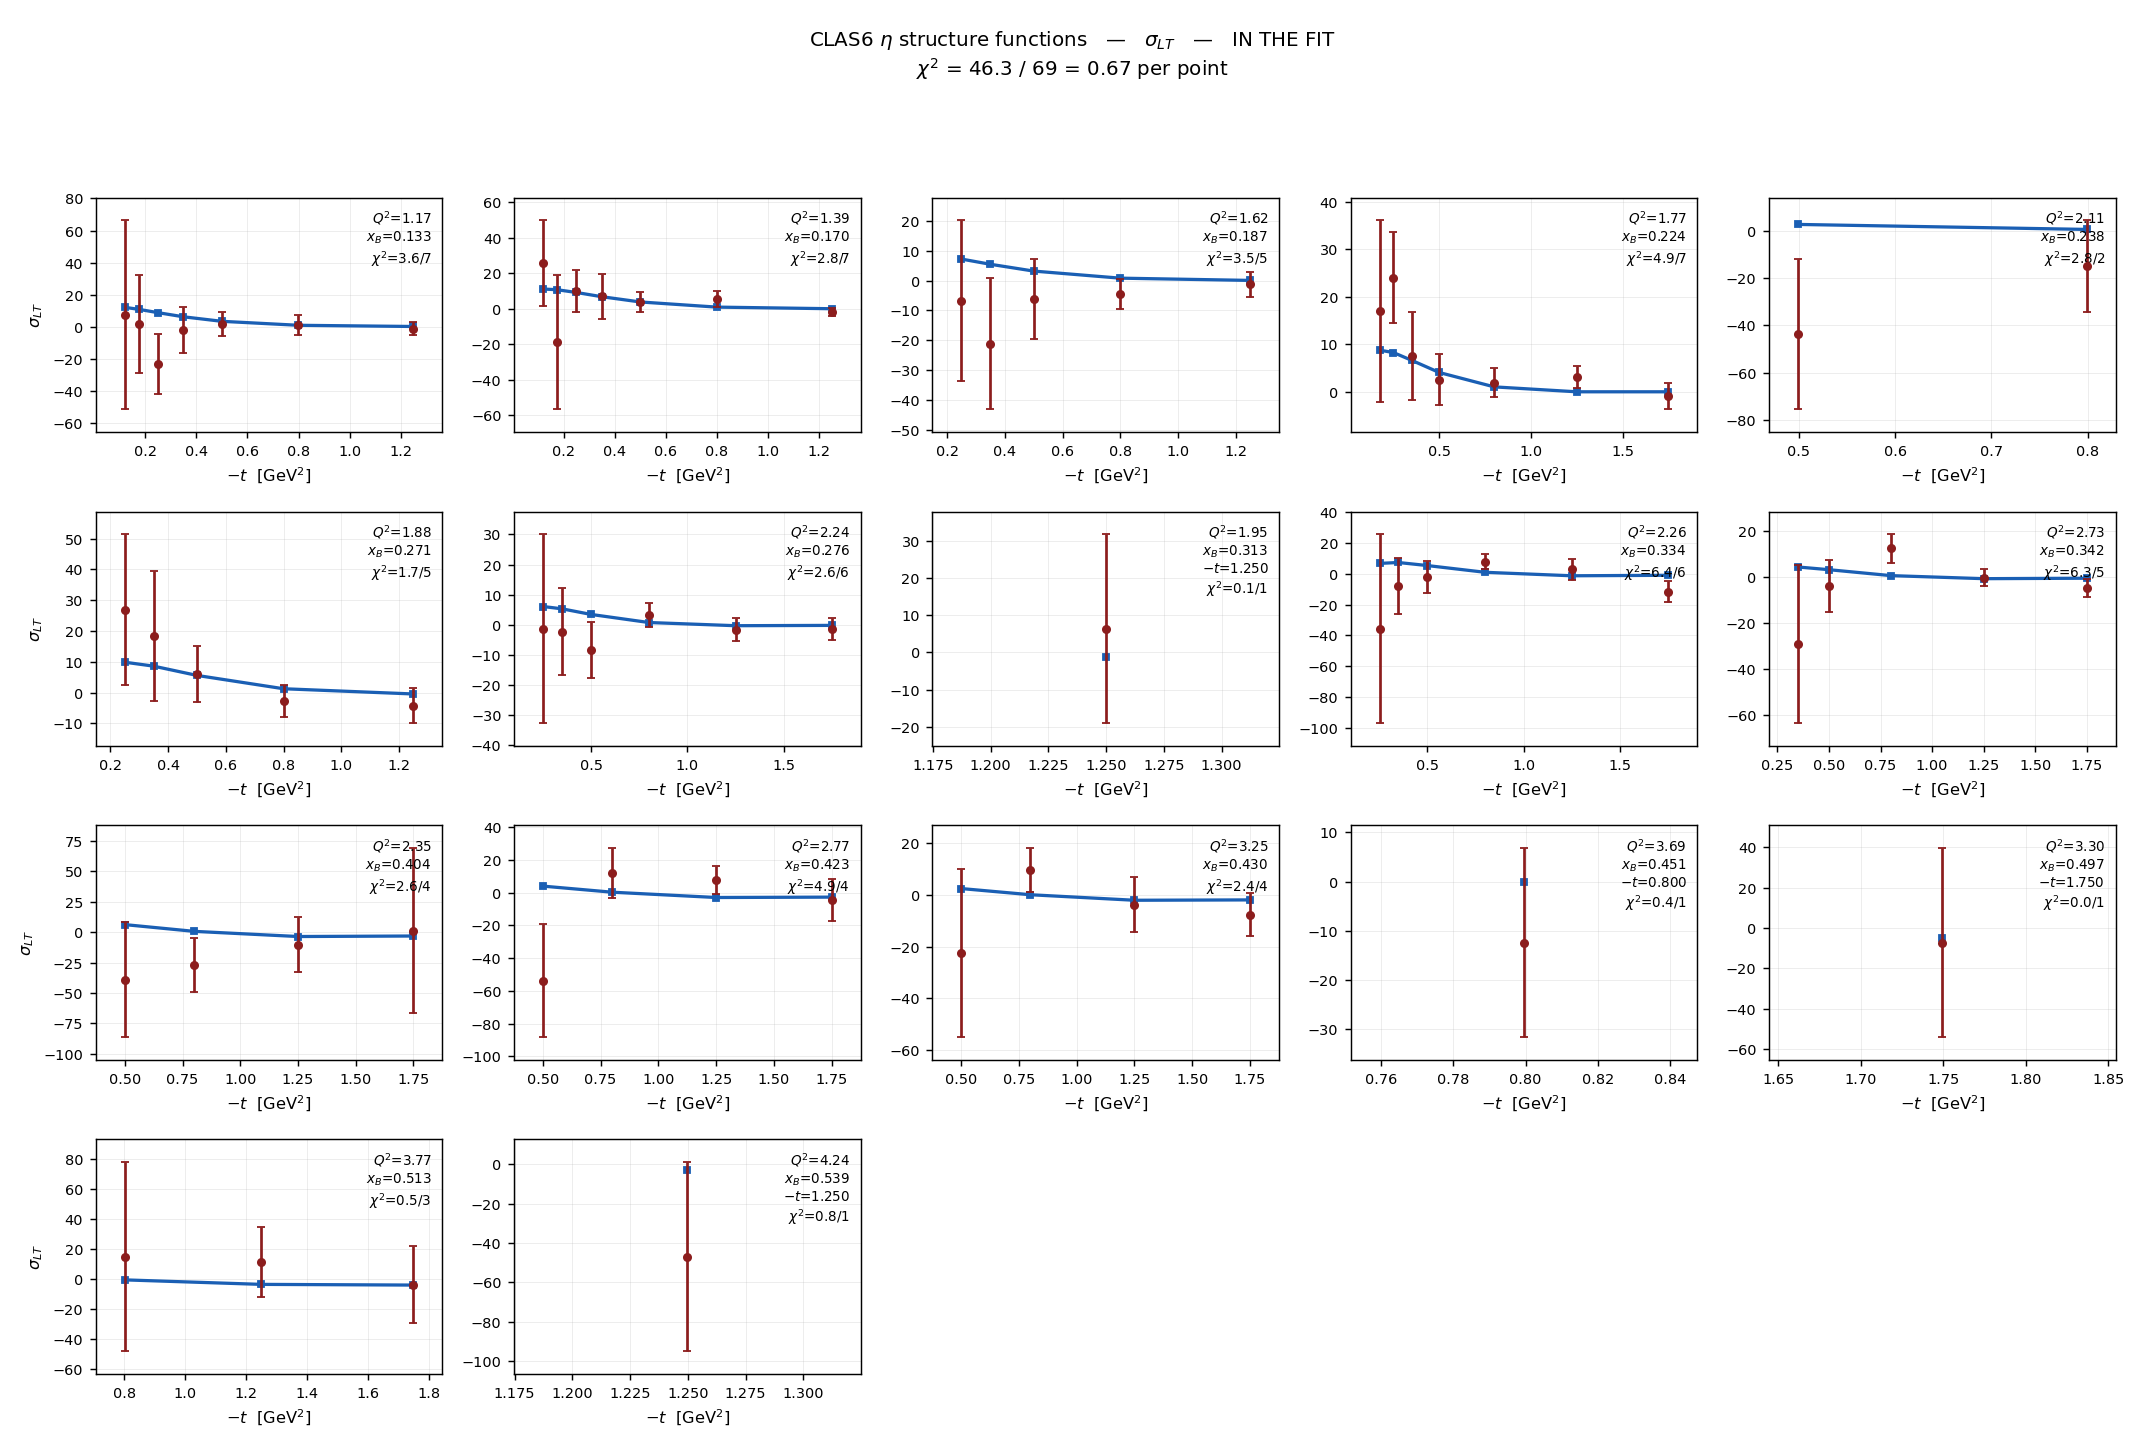
\includegraphics[width=\textwidth]{03_clas6_eta_in_LT.png}
\caption{CLAS6 $\eta$ off the proton --- $\sigma_{LT}$.  This set: $\chi^2 = 217.0/207 = 1.05$ per point.}
\end{figure}

\begin{figure}[p]\centering
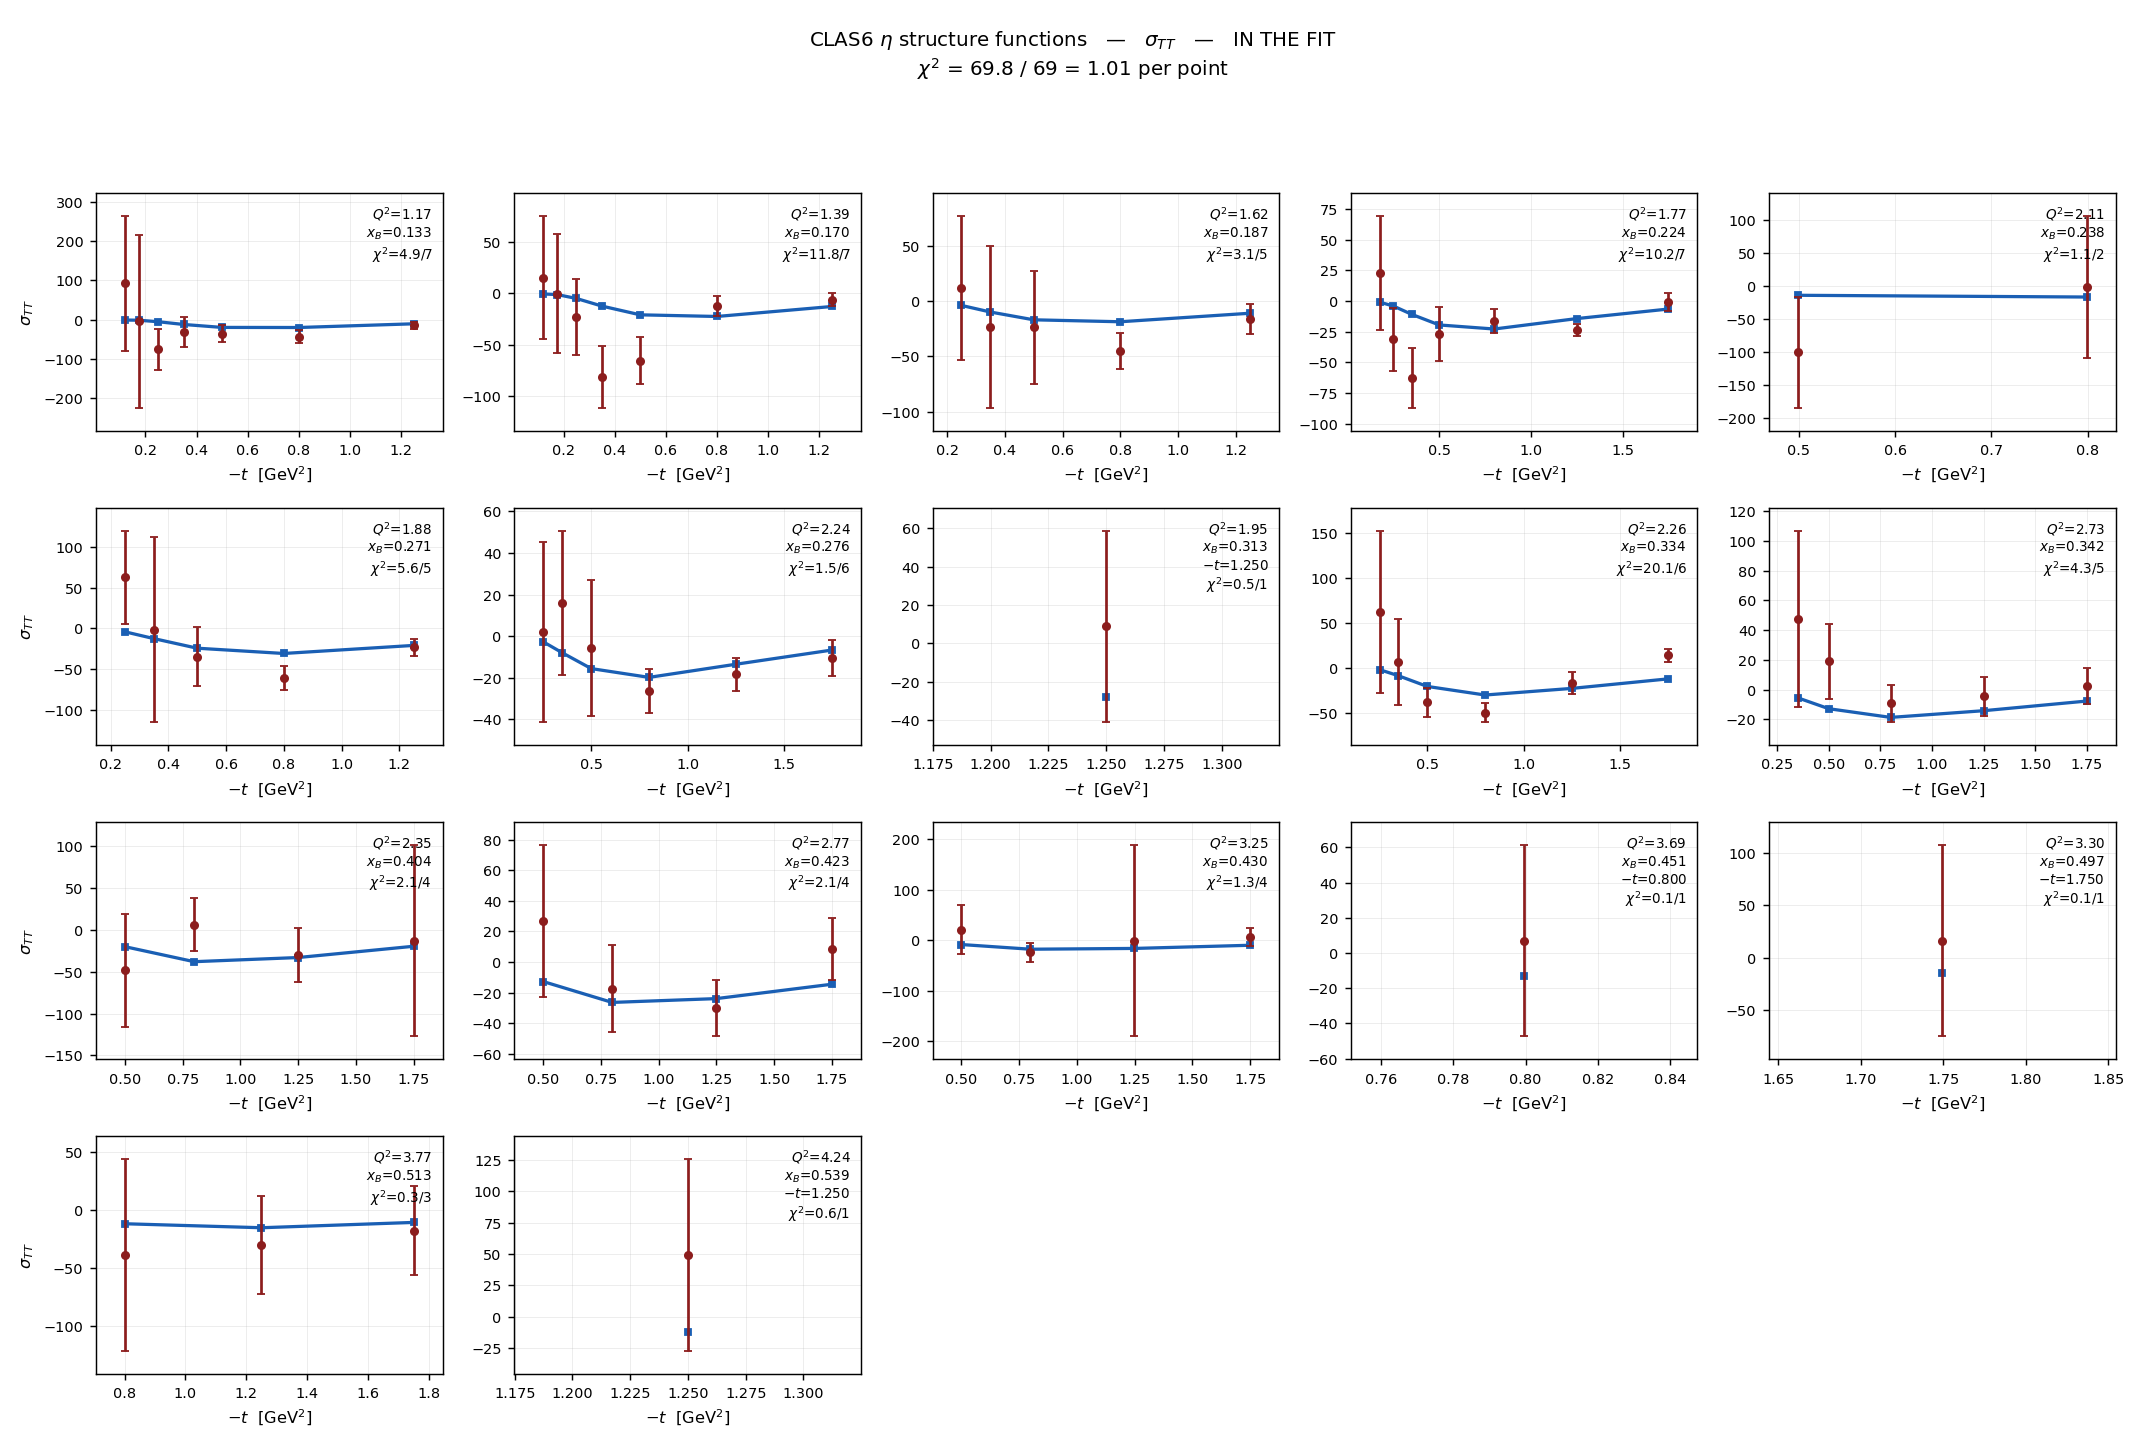
\includegraphics[width=\textwidth]{03_clas6_eta_in_TT.png}
\caption{CLAS6 $\eta$ off the proton --- $\sigma_{TT}$.  This set: $\chi^2 = 217.0/207 = 1.05$ per point.}
\end{figure}

\begin{figure}[p]\centering
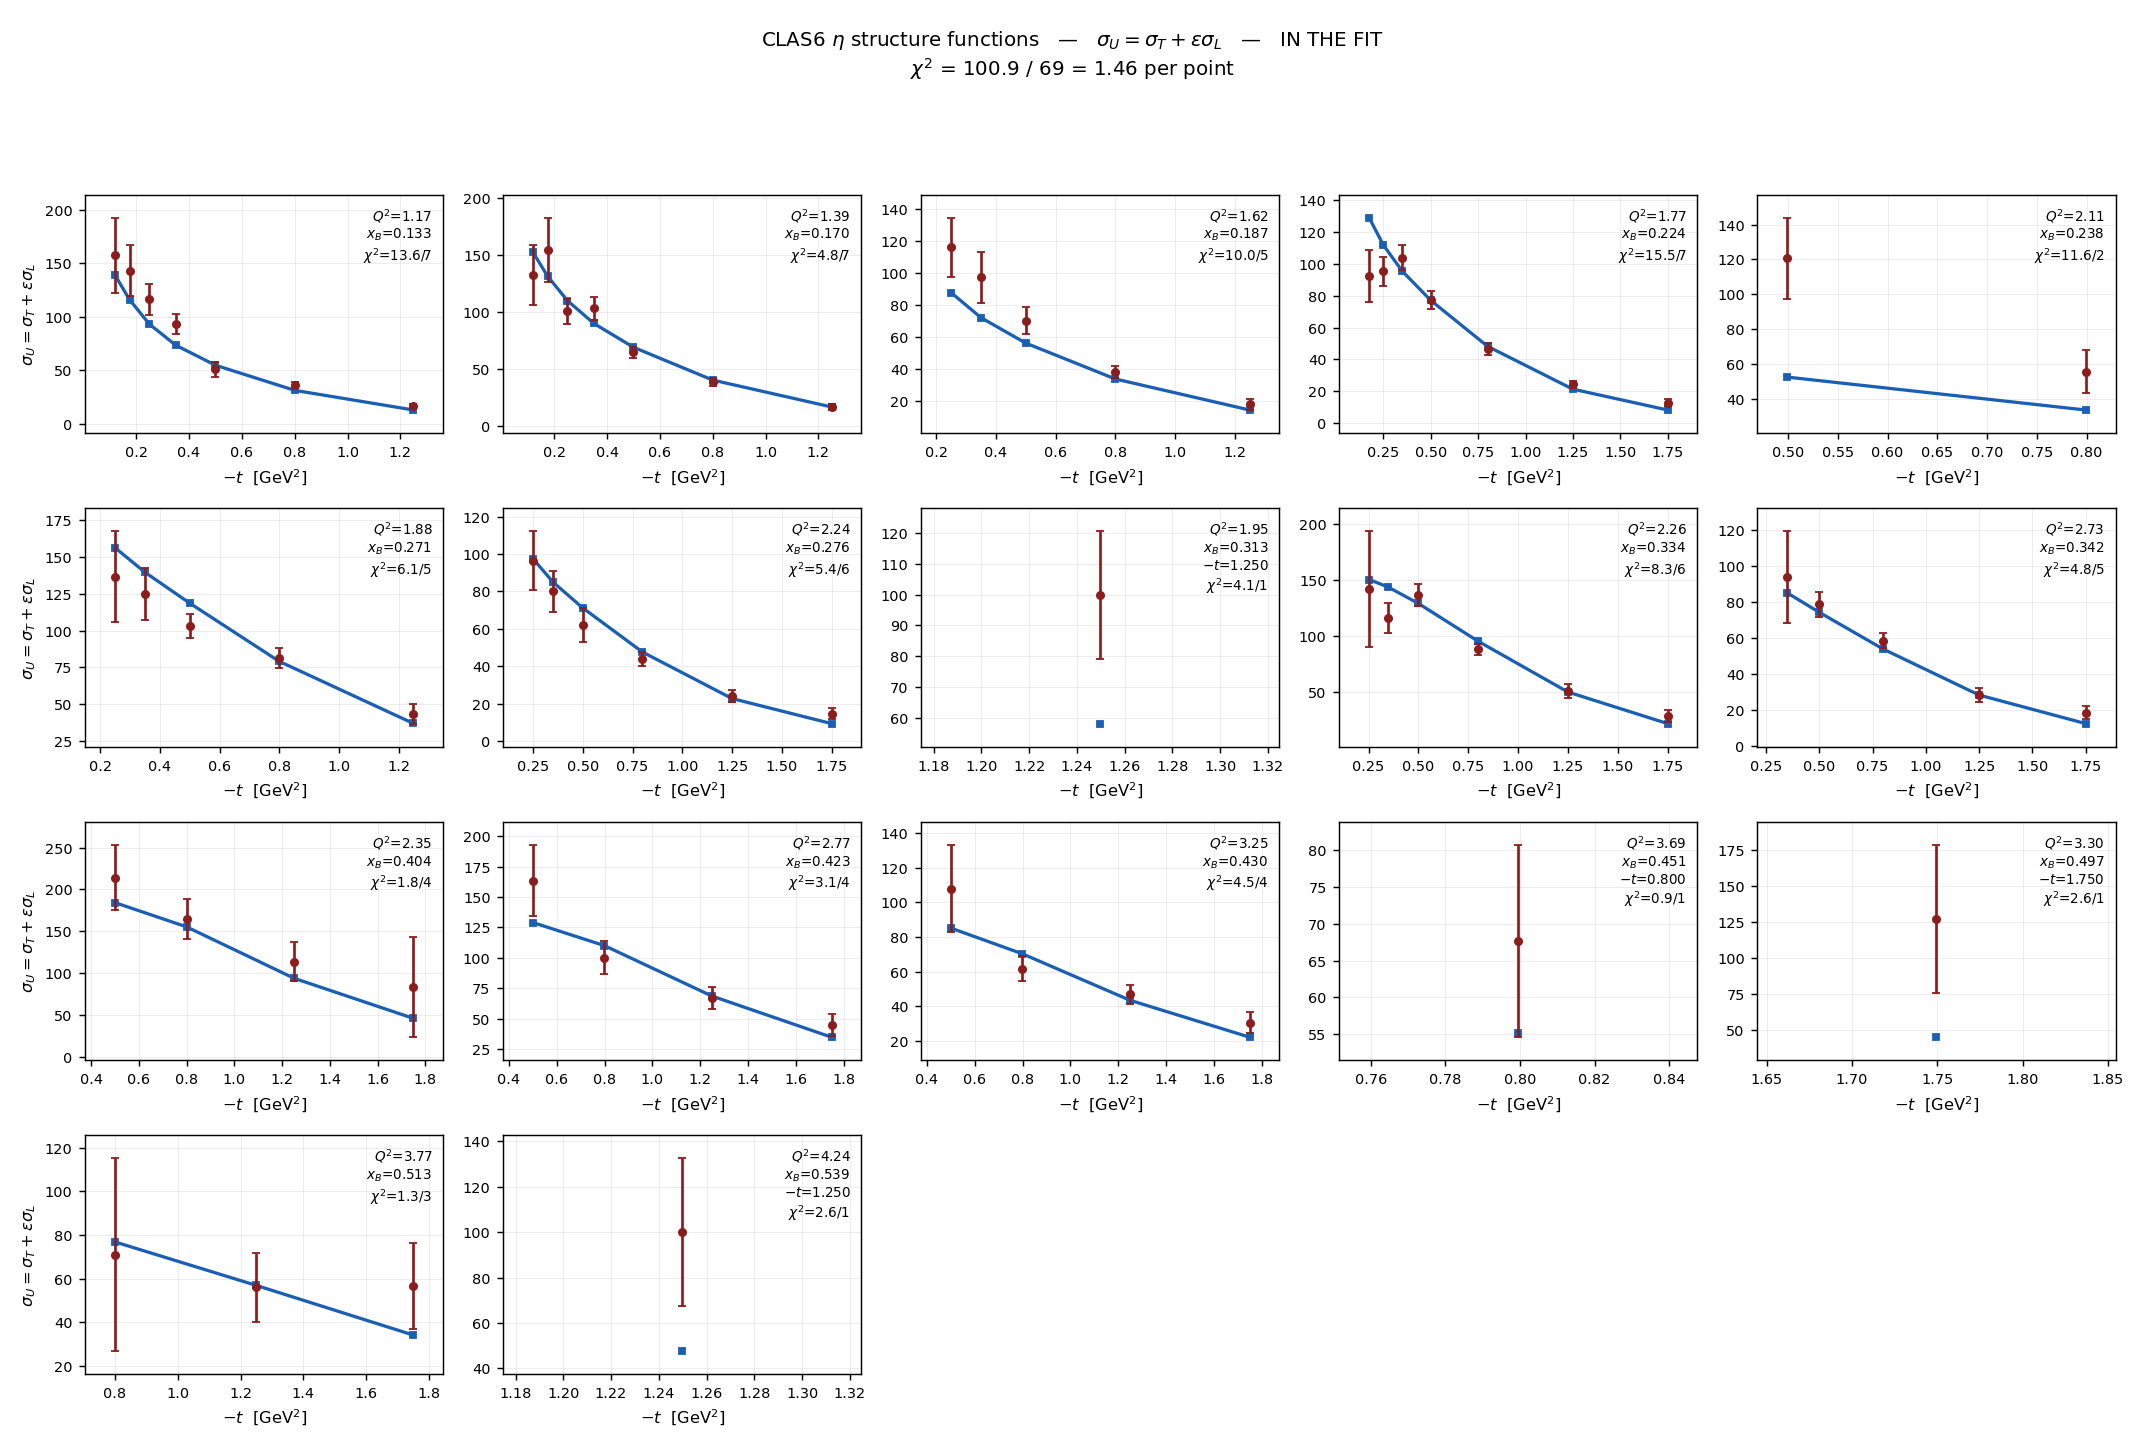
\includegraphics[width=\textwidth]{03_clas6_eta_in_U.png}
\caption{CLAS6 $\eta$ off the proton --- $\sigma_U=\sigma_T+\epsilon\sigma_L$.  This set: $\chi^2 = 217.0/207 = 1.05$ per point.}
\end{figure}

\begin{figure}[p]\centering
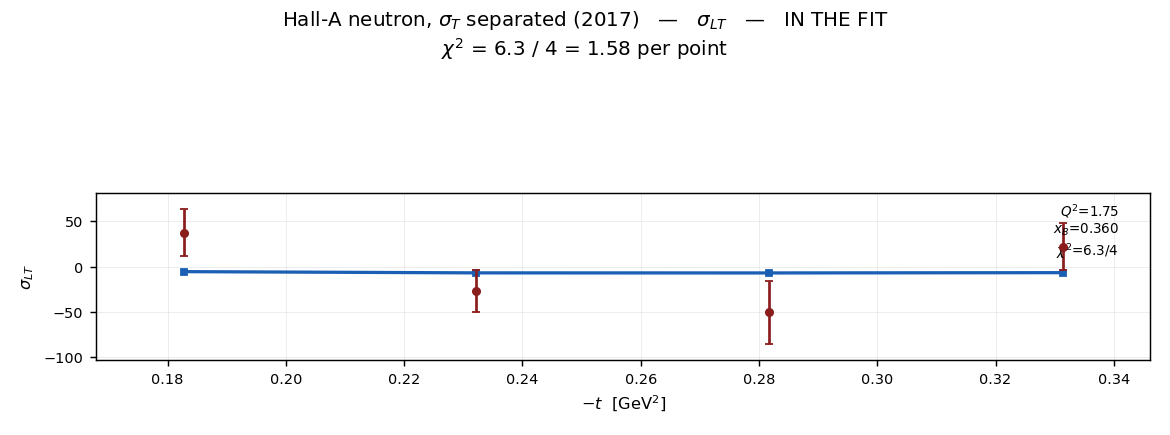
\includegraphics[width=\textwidth]{04_halla_n_in_LT.png}
\caption{Hall A 2017, $\pi^0$ off the NEUTRON --- $\sigma_{LT}$.  This set: $\chi^2 = 20.7/12 = 1.72$ per point.}
\end{figure}

\begin{figure}[p]\centering
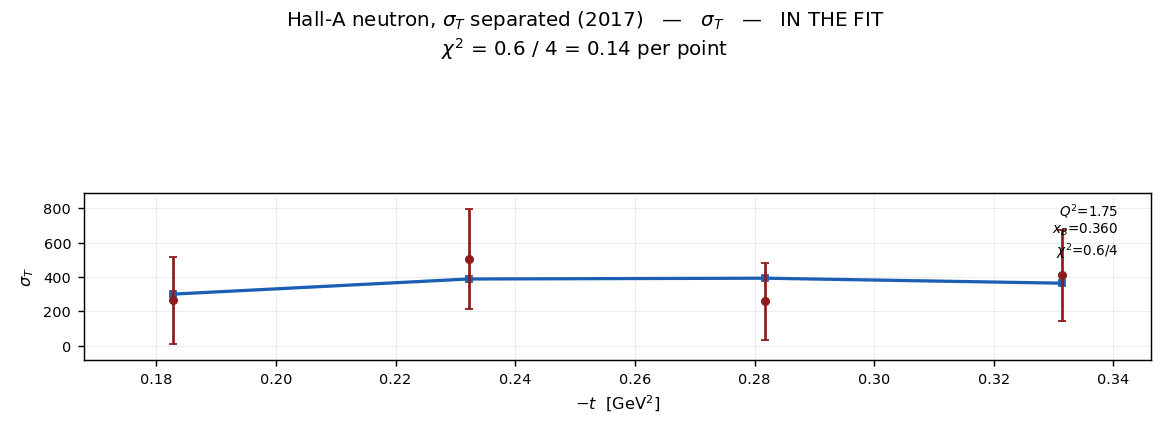
\includegraphics[width=\textwidth]{04_halla_n_in_T.png}
\caption{Hall A 2017, $\pi^0$ off the NEUTRON --- $\sigma_T$.  This set: $\chi^2 = 20.7/12 = 1.72$ per point.}
\end{figure}

\begin{figure}[p]\centering
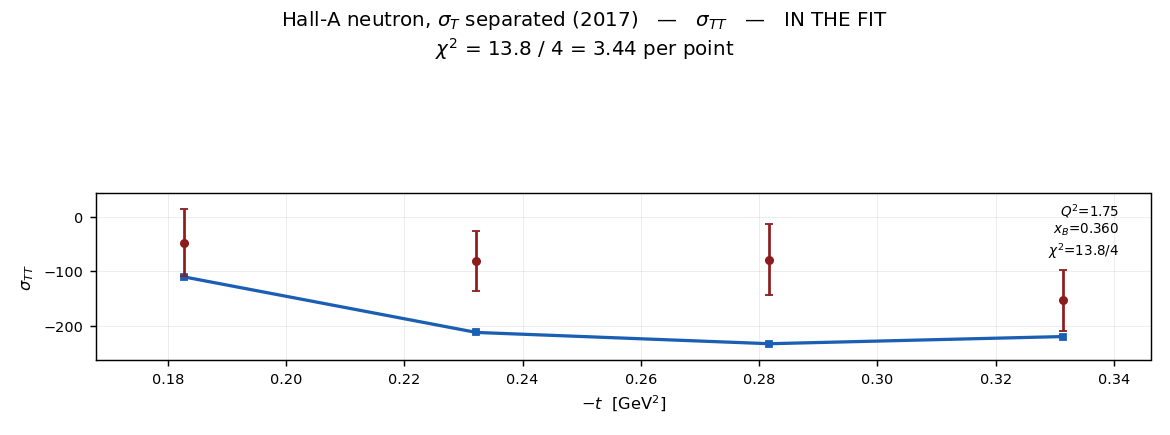
\includegraphics[width=\textwidth]{04_halla_n_in_TT.png}
\caption{Hall A 2017, $\pi^0$ off the NEUTRON --- $\sigma_{TT}$.  This set: $\chi^2 = 20.7/12 = 1.72$ per point.}
\end{figure}

\begin{figure}[p]\centering
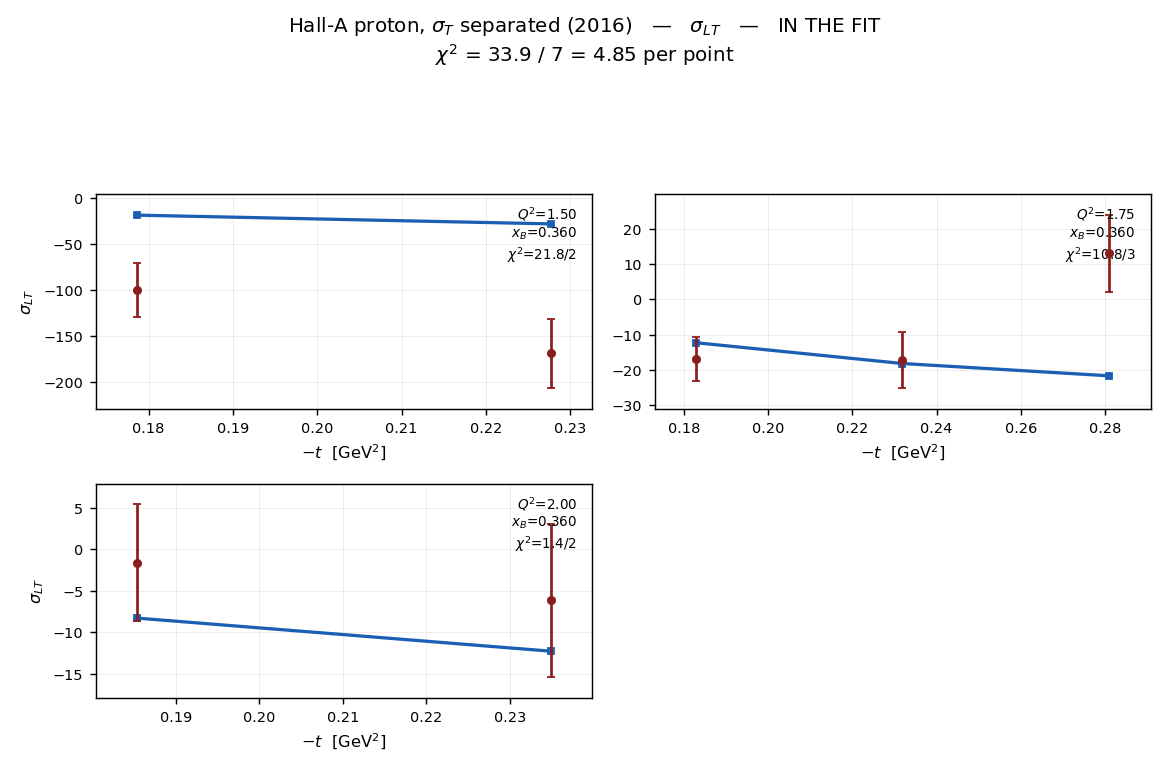
\includegraphics[width=\textwidth]{05_halla_y16_in_LT.png}
\caption{Hall A 2016, Rosenbluth separated --- $\sigma_{LT}$.  This set: $\chi^2 = 95.3/21 = 4.54$ per point.}
\end{figure}

\begin{figure}[p]\centering
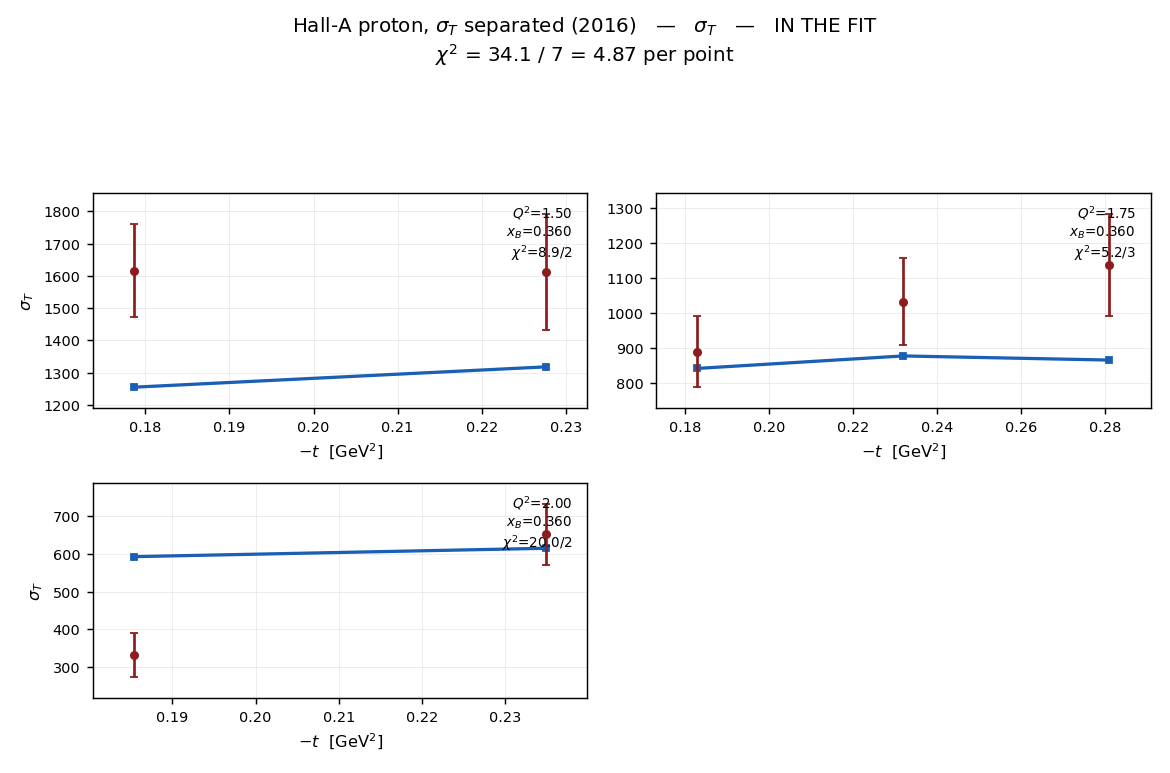
\includegraphics[width=\textwidth]{05_halla_y16_in_T.png}
\caption{Hall A 2016, Rosenbluth separated --- $\sigma_T$.  This set: $\chi^2 = 95.3/21 = 4.54$ per point.}
\end{figure}

\begin{figure}[p]\centering
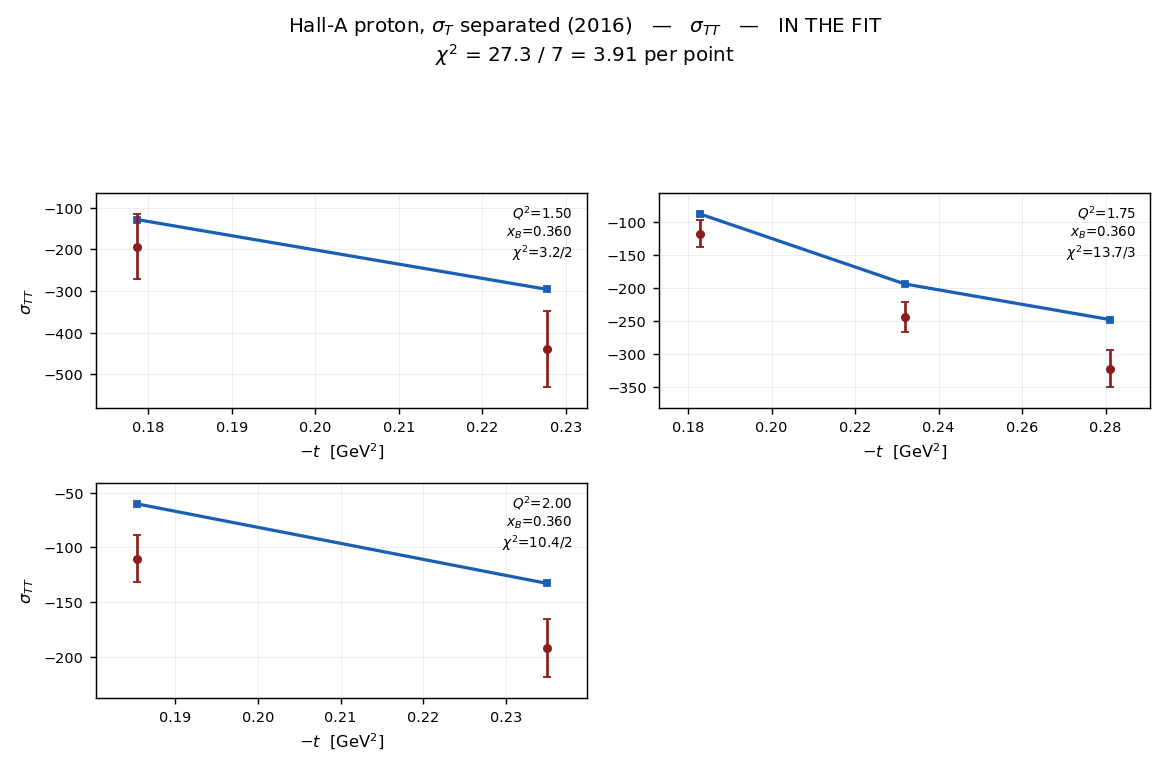
\includegraphics[width=\textwidth]{05_halla_y16_in_TT.png}
\caption{Hall A 2016, Rosenbluth separated --- $\sigma_{TT}$.  This set: $\chi^2 = 95.3/21 = 4.54$ per point.}
\end{figure}

\begin{figure}[p]\centering
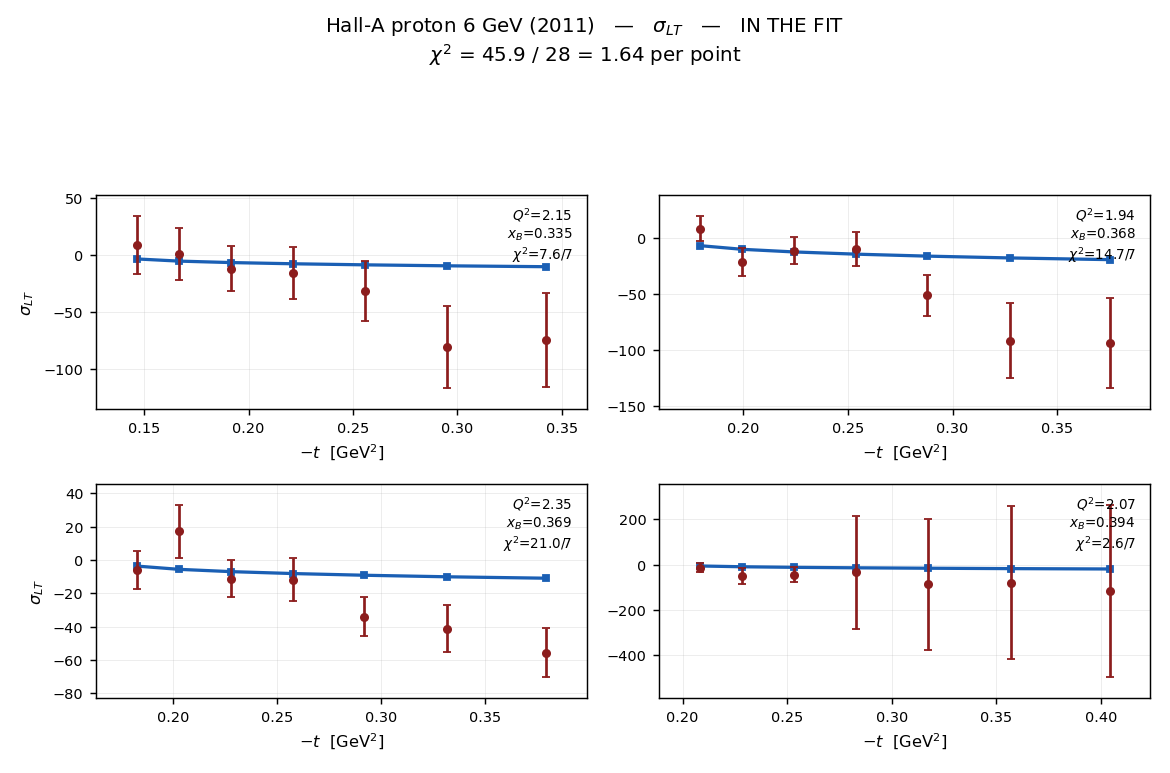
\includegraphics[width=\textwidth]{06_halla_y11_in_LT.png}
\caption{Hall A 2011 --- $\sigma_{LT}$.  This set: $\chi^2 = 143.3/112 = 1.28$ per point.}
\end{figure}

\begin{figure}[p]\centering
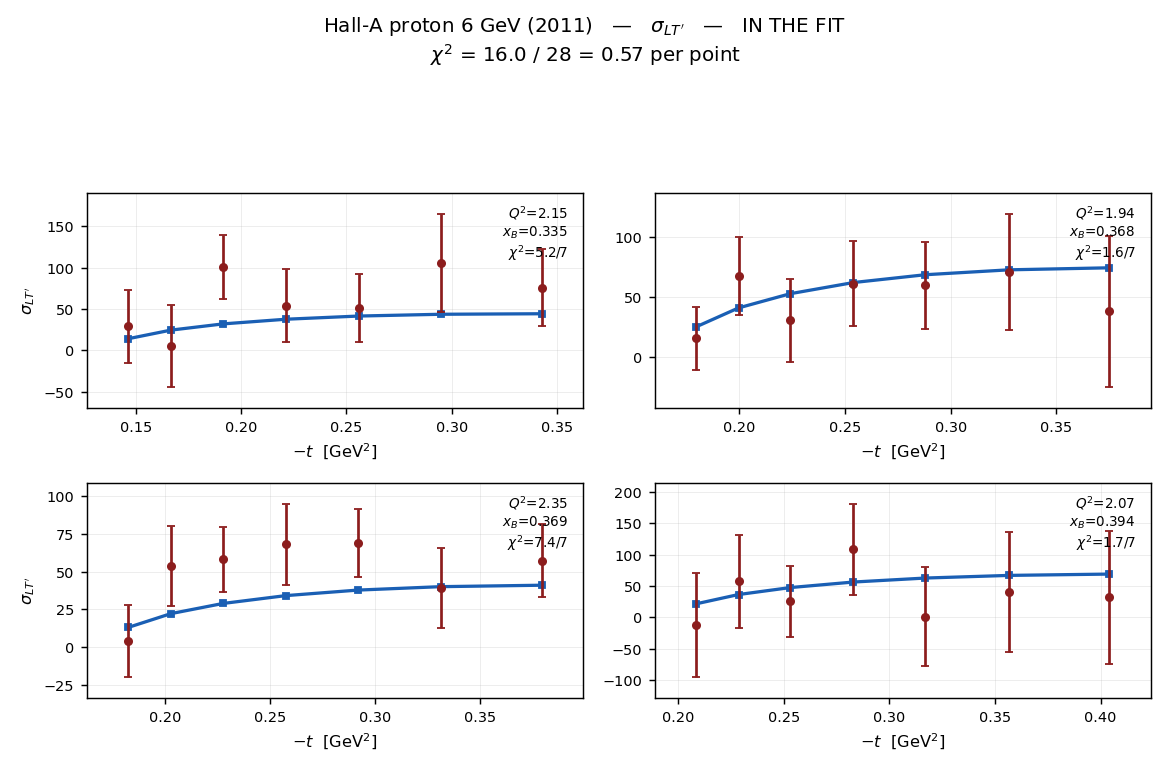
\includegraphics[width=\textwidth]{06_halla_y11_in_LTp.png}
\caption{Hall A 2011 --- $\sigma_{LT^\prime}$.  This set: $\chi^2 = 143.3/112 = 1.28$ per point.}
\end{figure}

\begin{figure}[p]\centering
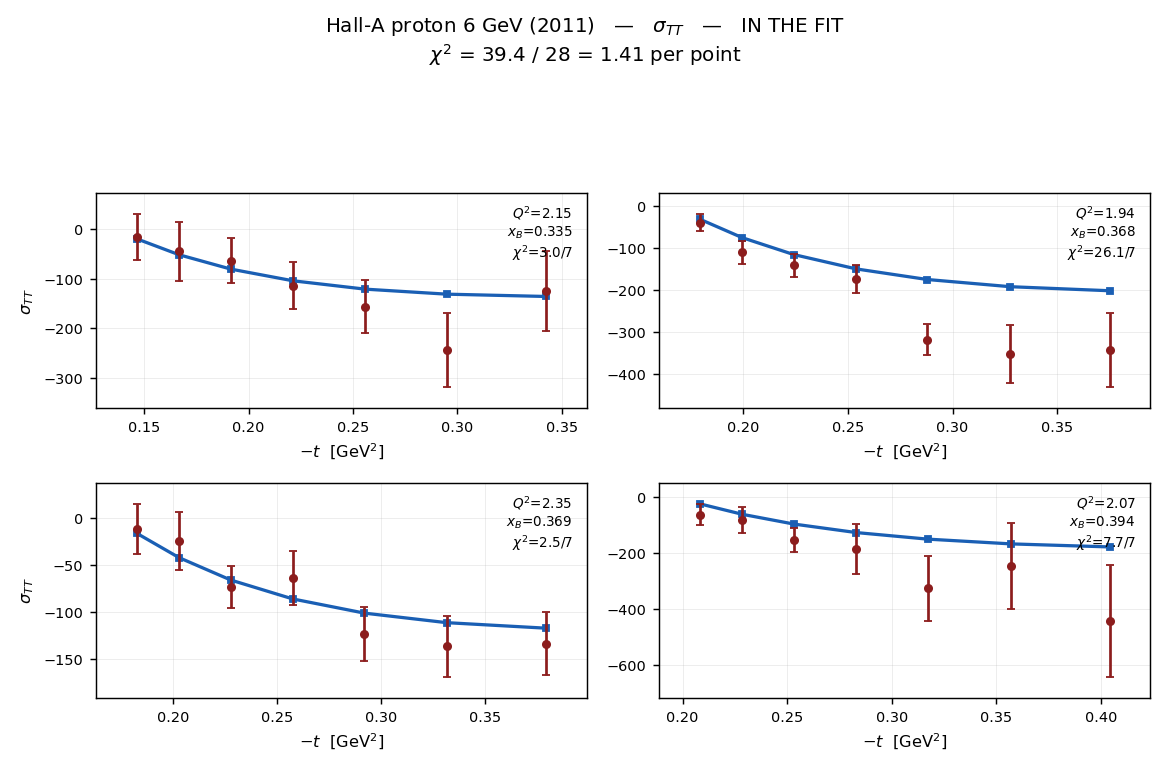
\includegraphics[width=\textwidth]{06_halla_y11_in_TT.png}
\caption{Hall A 2011 --- $\sigma_{TT}$.  This set: $\chi^2 = 143.3/112 = 1.28$ per point.}
\end{figure}

\begin{figure}[p]\centering
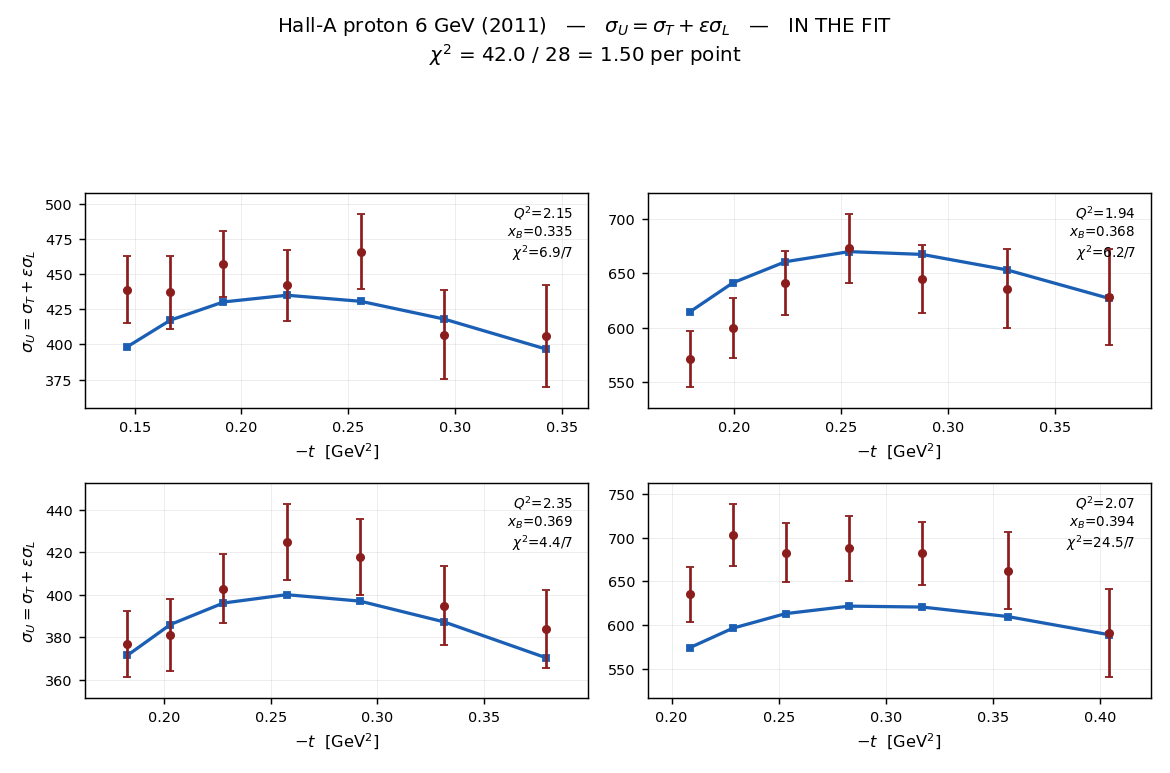
\includegraphics[width=\textwidth]{06_halla_y11_in_U.png}
\caption{Hall A 2011 --- $\sigma_U=\sigma_T+\epsilon\sigma_L$.  This set: $\chi^2 = 143.3/112 = 1.28$ per point.}
\end{figure}

\begin{figure}[p]\centering
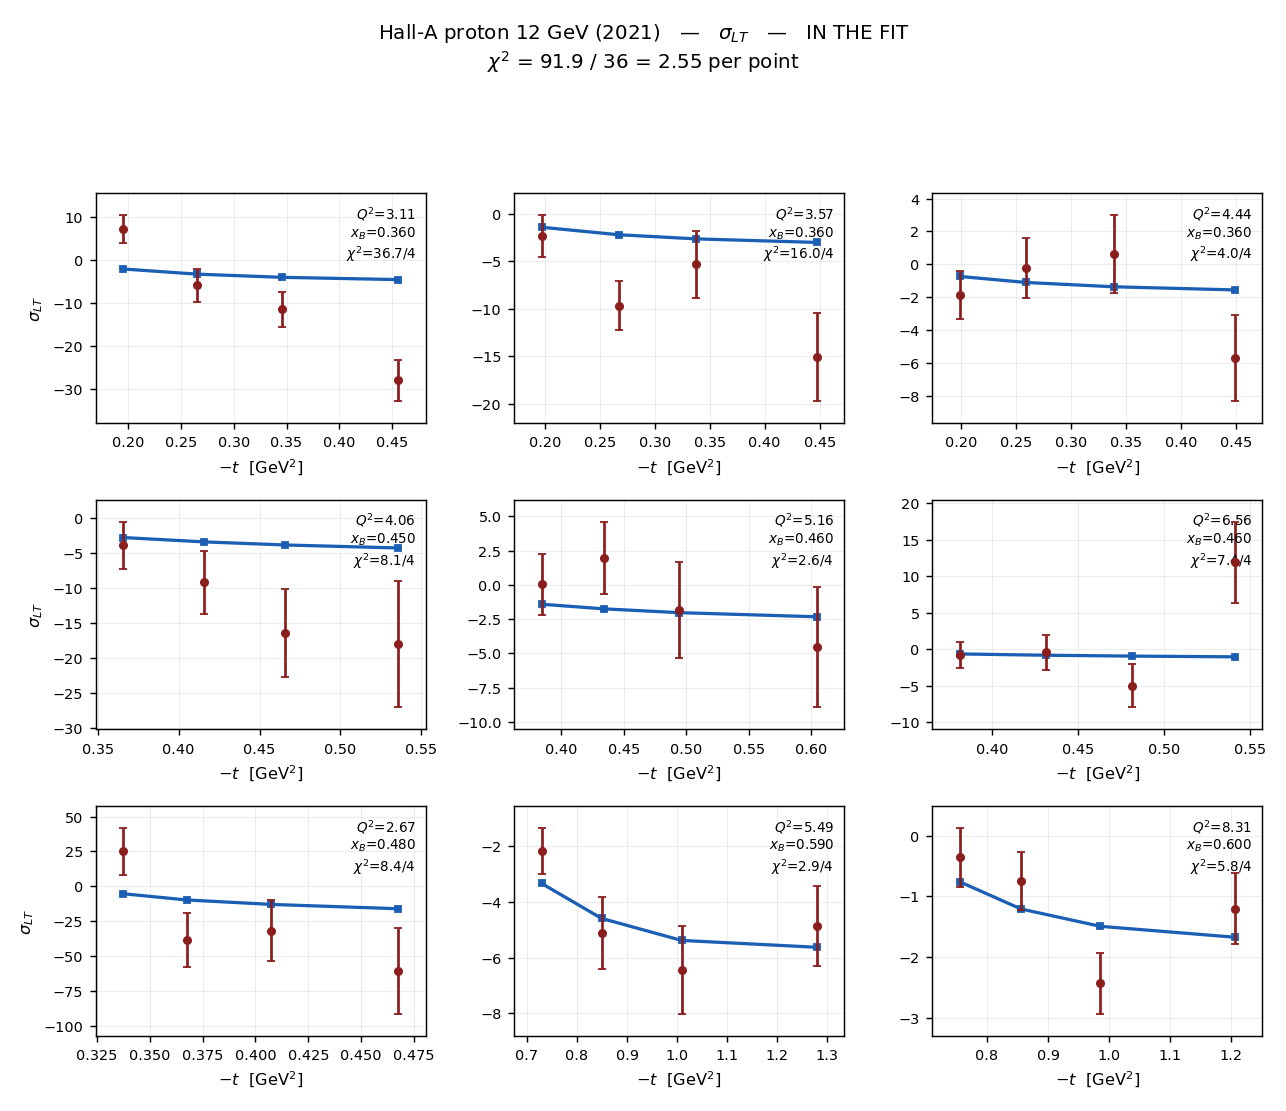
\includegraphics[width=\textwidth]{07_halla_y21_in_LT.png}
\caption{Hall A 2021, the only data above $Q^2=4.3$ --- $\sigma_{LT}$.  This set: $\chi^2 = 358.2/144 = 2.49$ per point.}
\end{figure}

\begin{figure}[p]\centering
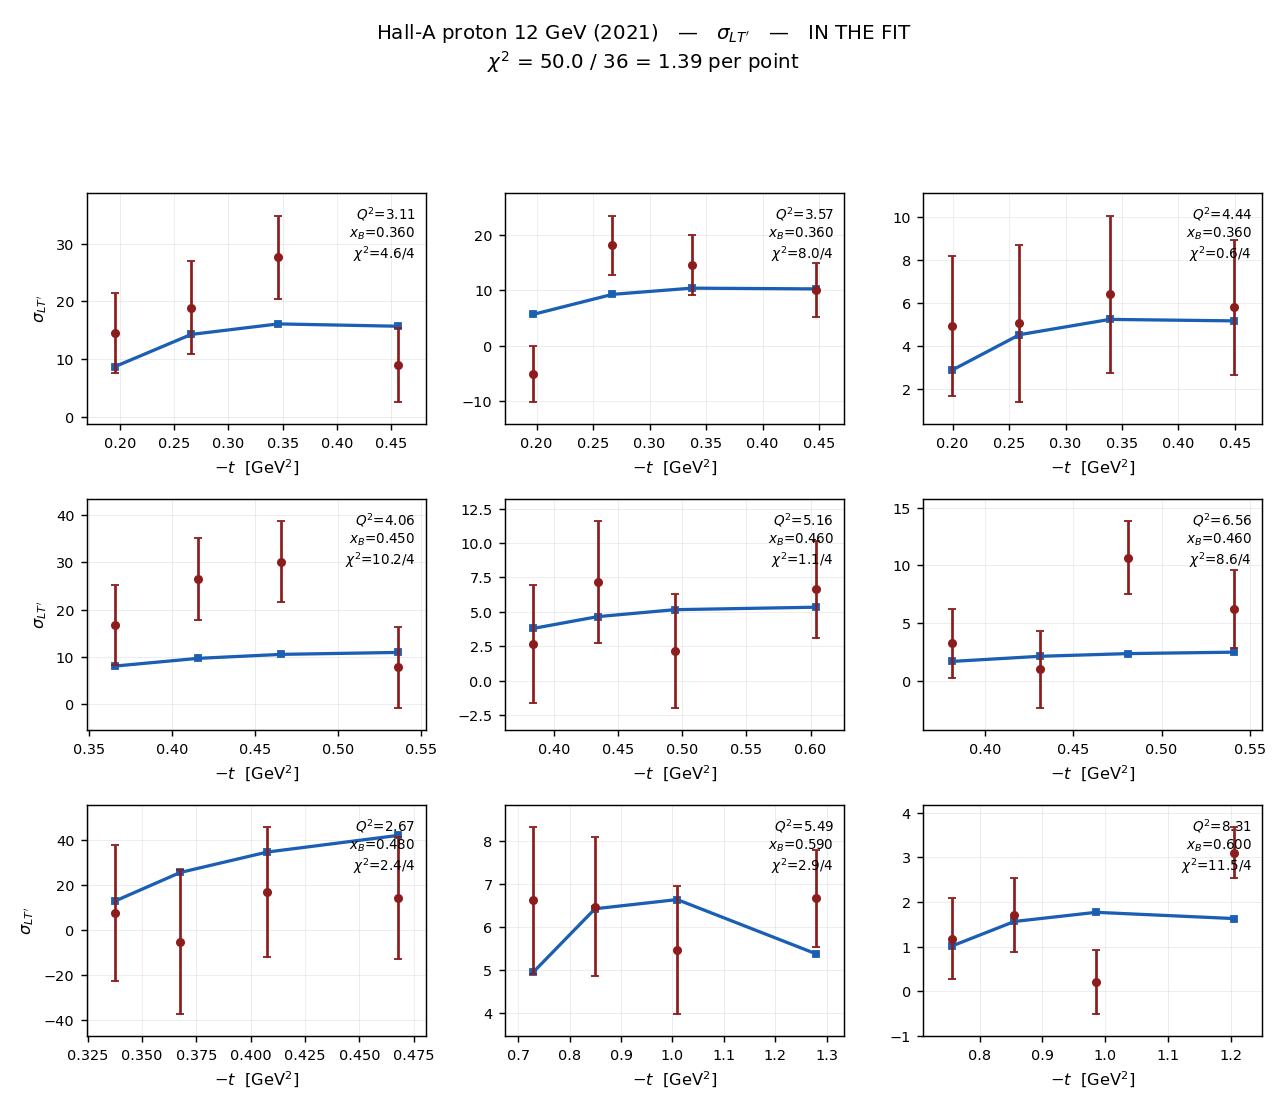
\includegraphics[width=\textwidth]{07_halla_y21_in_LTp.png}
\caption{Hall A 2021, the only data above $Q^2=4.3$ --- $\sigma_{LT^\prime}$.  This set: $\chi^2 = 358.2/144 = 2.49$ per point.}
\end{figure}

\begin{figure}[p]\centering
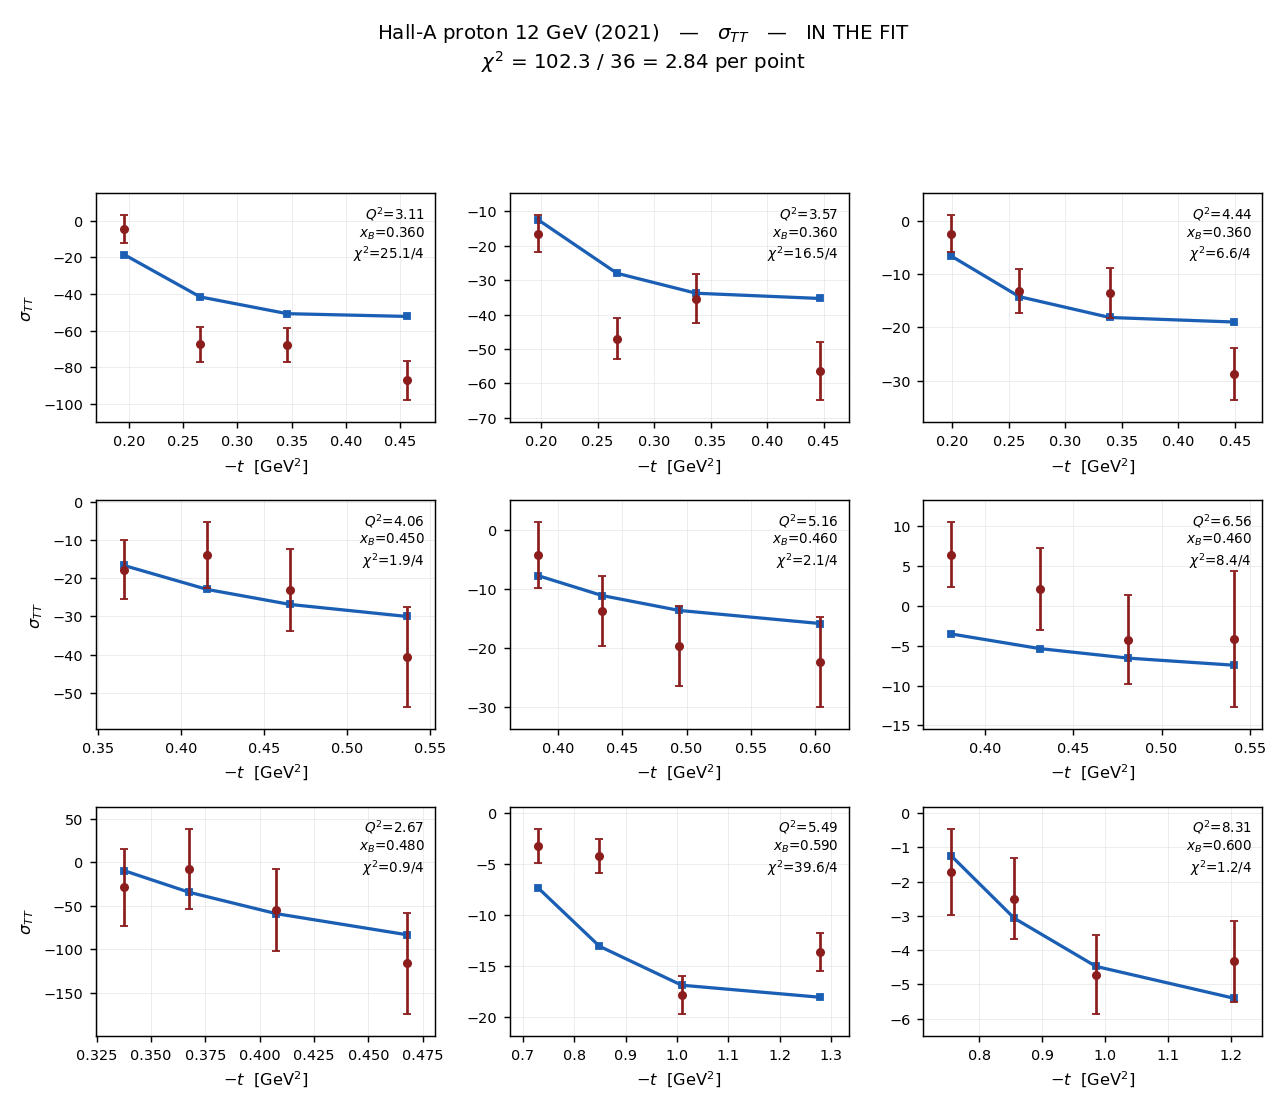
\includegraphics[width=\textwidth]{07_halla_y21_in_TT.png}
\caption{Hall A 2021, the only data above $Q^2=4.3$ --- $\sigma_{TT}$.  This set: $\chi^2 = 358.2/144 = 2.49$ per point.}
\end{figure}

\begin{figure}[p]\centering
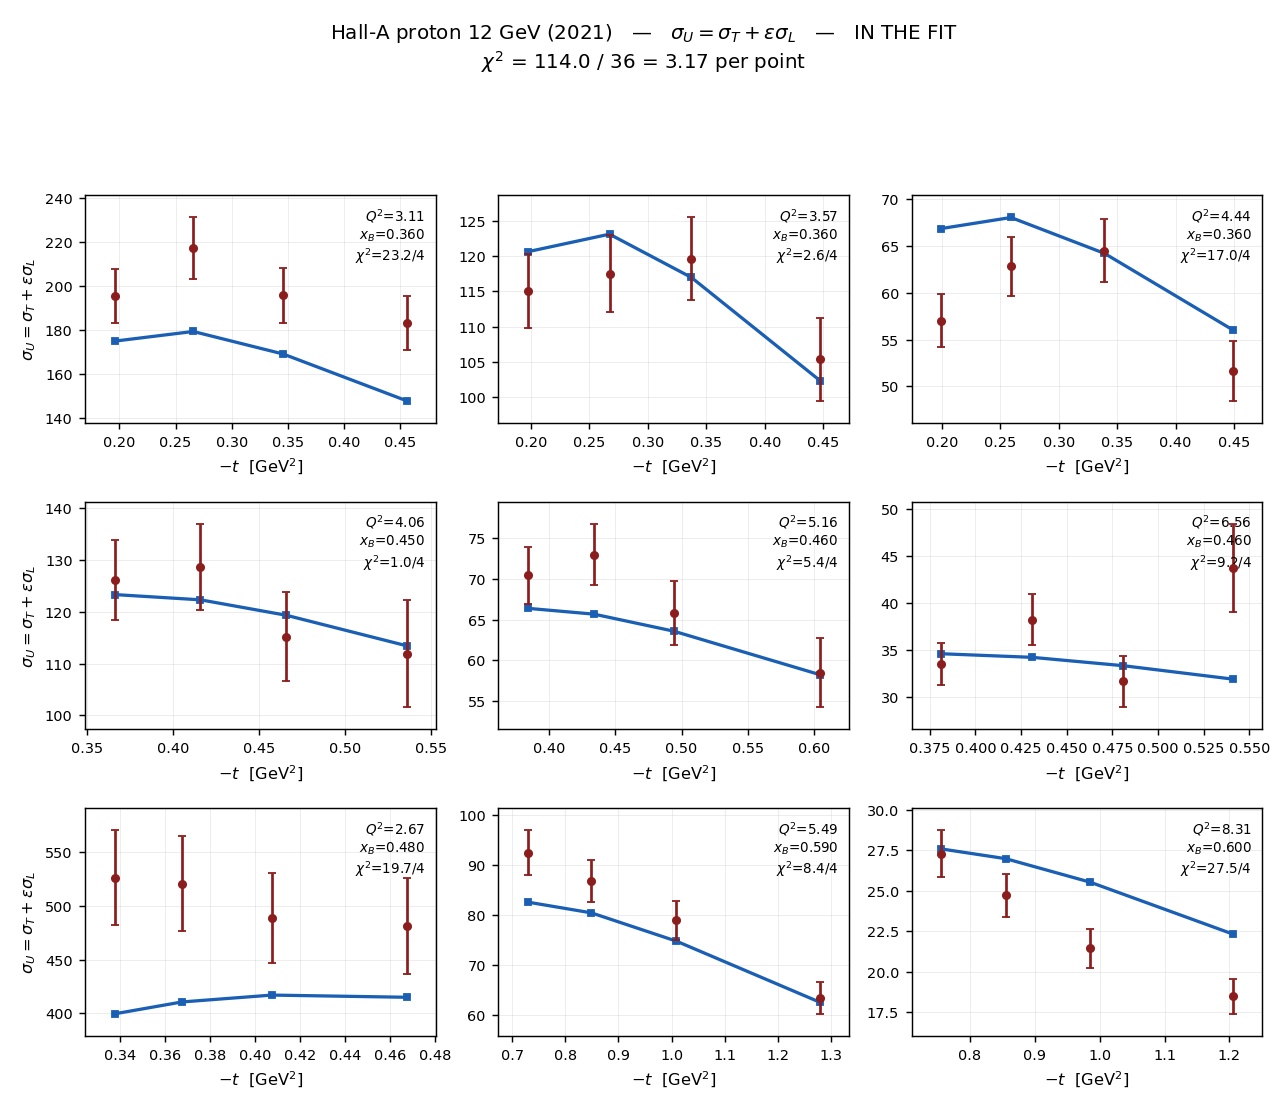
\includegraphics[width=\textwidth]{07_halla_y21_in_U.png}
\caption{Hall A 2021, the only data above $Q^2=4.3$ --- $\sigma_U=\sigma_T+\epsilon\sigma_L$.  This set: $\chi^2 = 358.2/144 = 2.49$ per point.}
\end{figure}

\begin{figure}[p]\centering
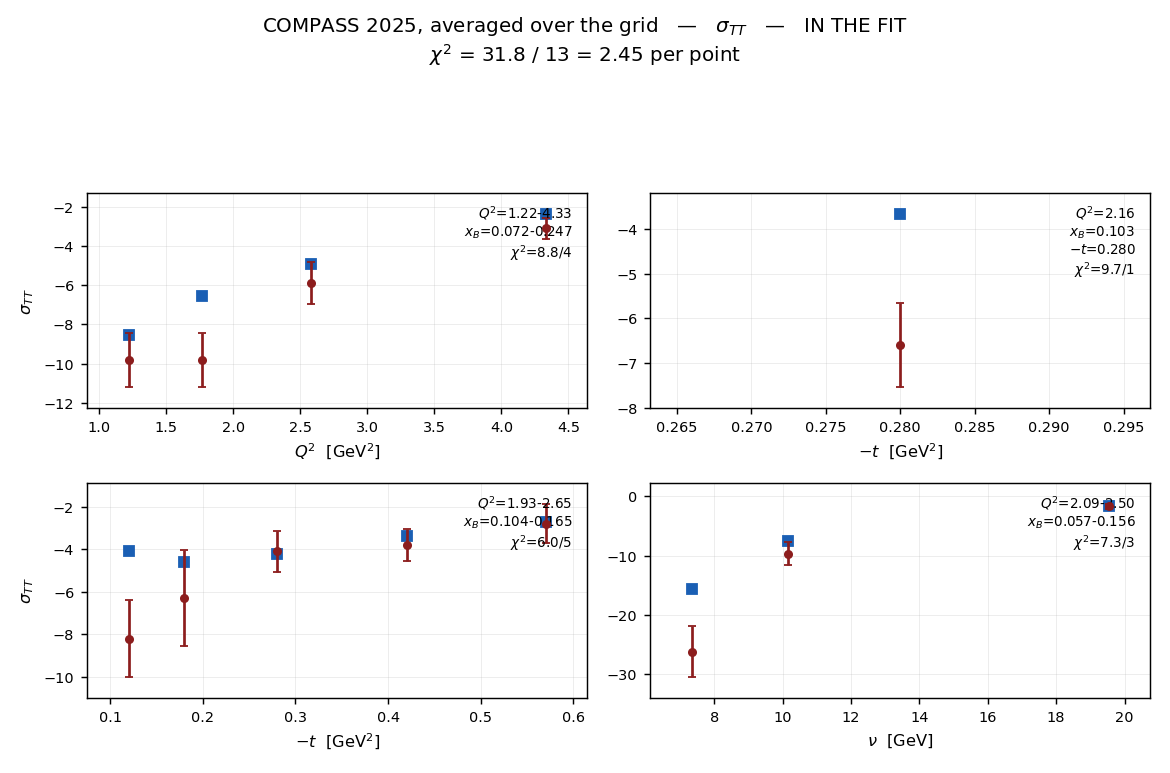
\includegraphics[width=\textwidth]{09_compass_in_TT.png}
\caption{COMPASS 2025, model averaged over the grid --- $\sigma_{TT}$.  This set: $\chi^2 = 65.4/26 = 2.51$ per point.}
\end{figure}

\begin{figure}[p]\centering
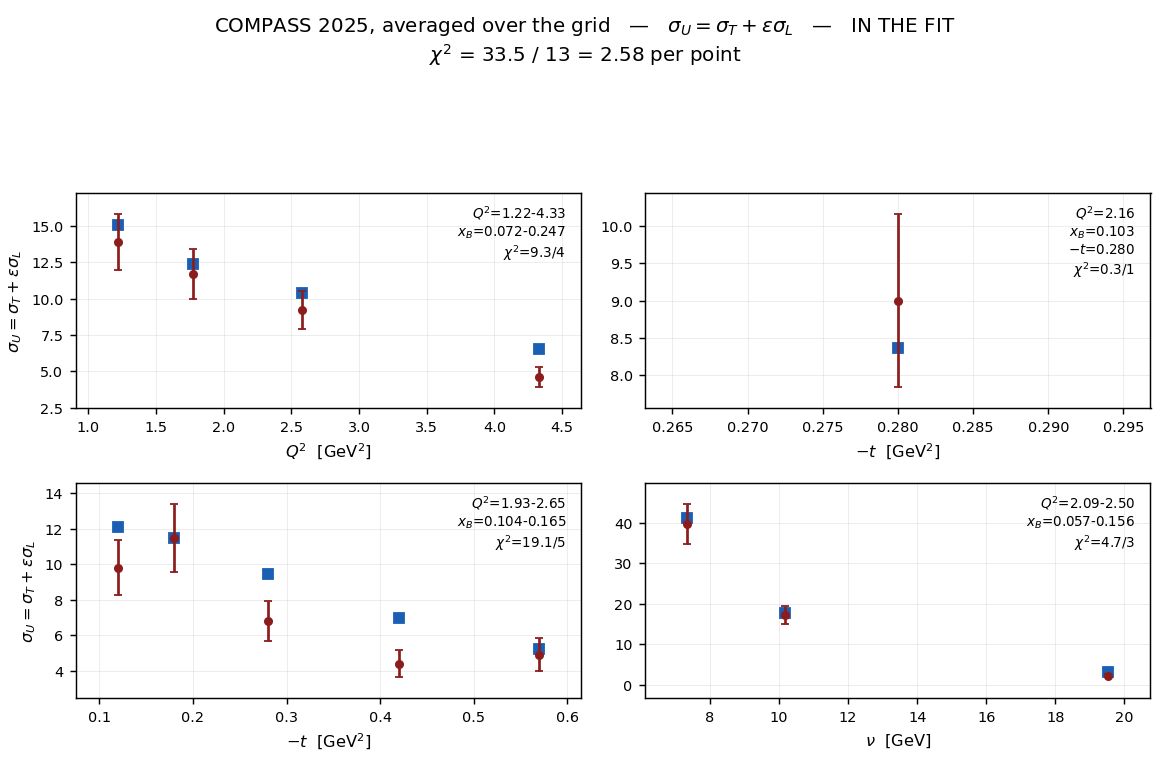
\includegraphics[width=\textwidth]{09_compass_in_U.png}
\caption{COMPASS 2025, model averaged over the grid --- $\sigma_U=\sigma_T+\epsilon\sigma_L$.  This set: $\chi^2 = 65.4/26 = 2.51$ per point.}
\end{figure}

\begin{figure}[p]\centering
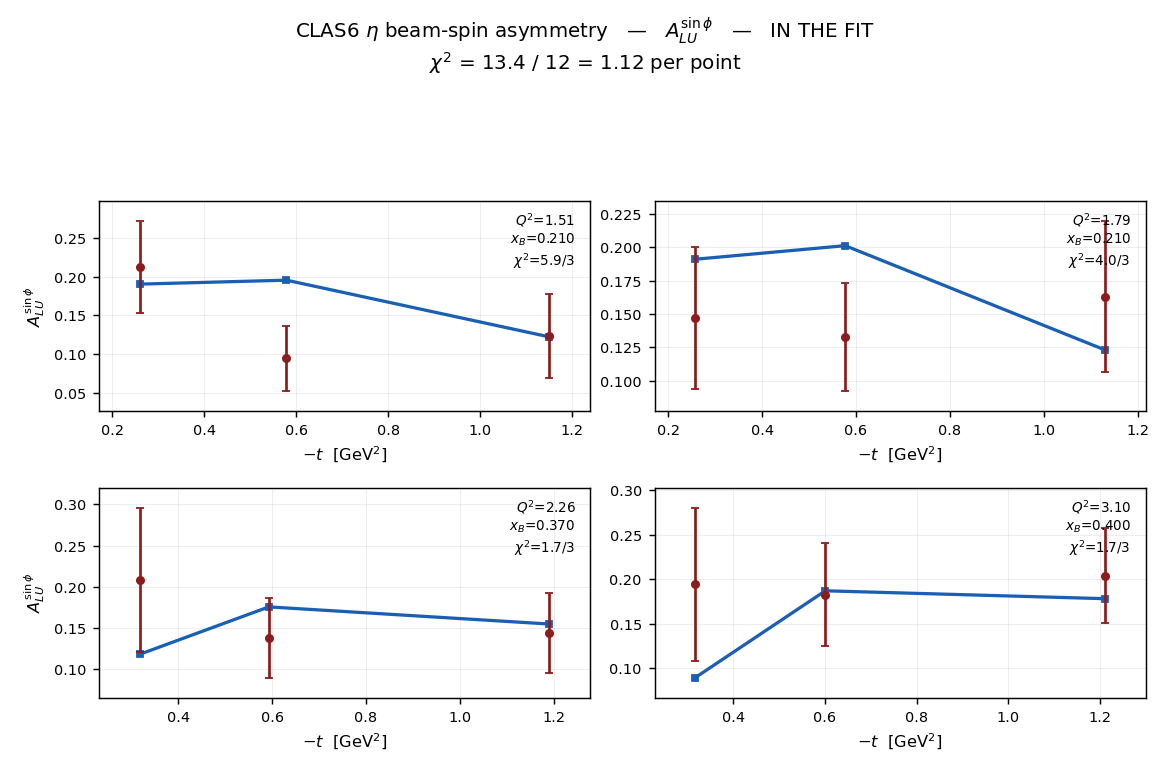
\includegraphics[width=\textwidth]{11_bsa_zhao_in_A_LUsinphi.png}
\caption{Zhao, $\eta$ beam-spin asymmetry --- $A_{LU}^{\sin\phi}$.  This set: $\chi^2 = 13.4/12 = 1.12$ per point.}
\end{figure}

\begin{figure}[p]\centering
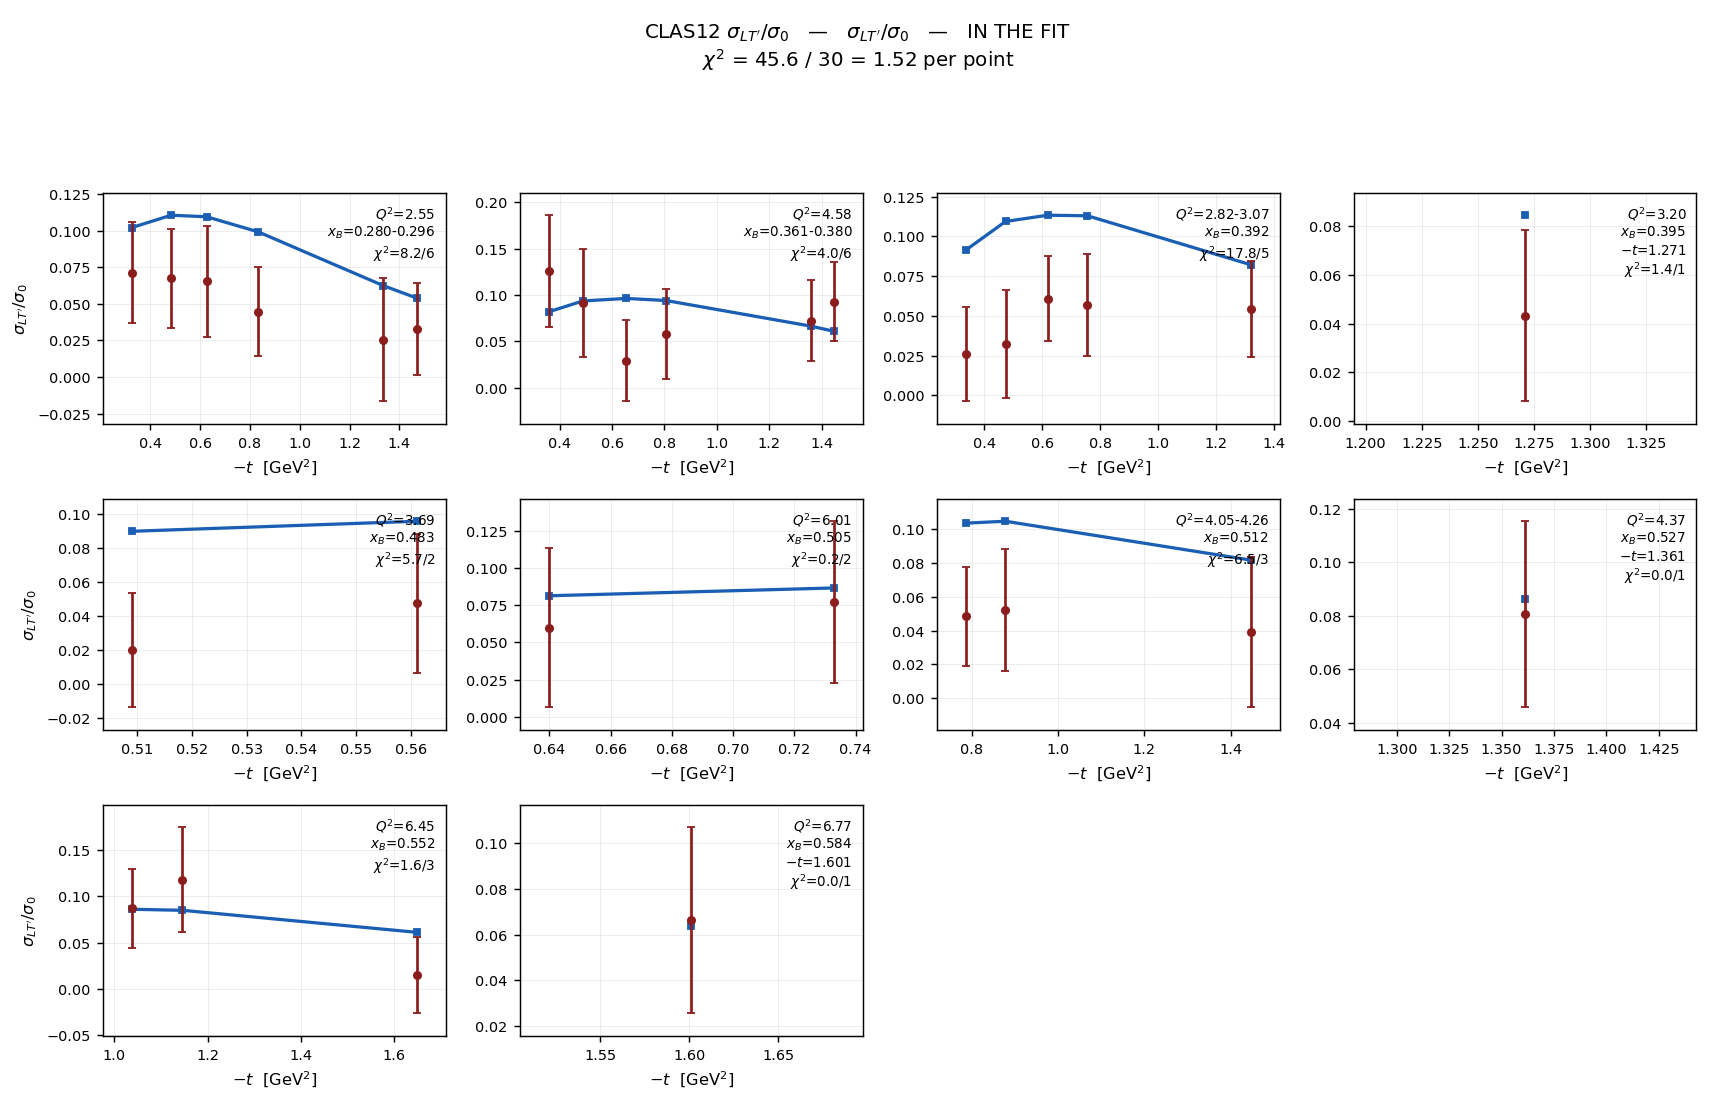
\includegraphics[width=\textwidth]{12_bsa_clas12_in_sigma_LTp_over_sigma_0.png}
\caption{CLAS12 $\sigma_{LT^\prime}/\sigma_0$ --- $\sigma_{LT^\prime}/\sigma_0$.  This set: $\chi^2 = 45.6/30 = 1.52$ per point.}
\end{figure}

\begin{figure}[p]\centering
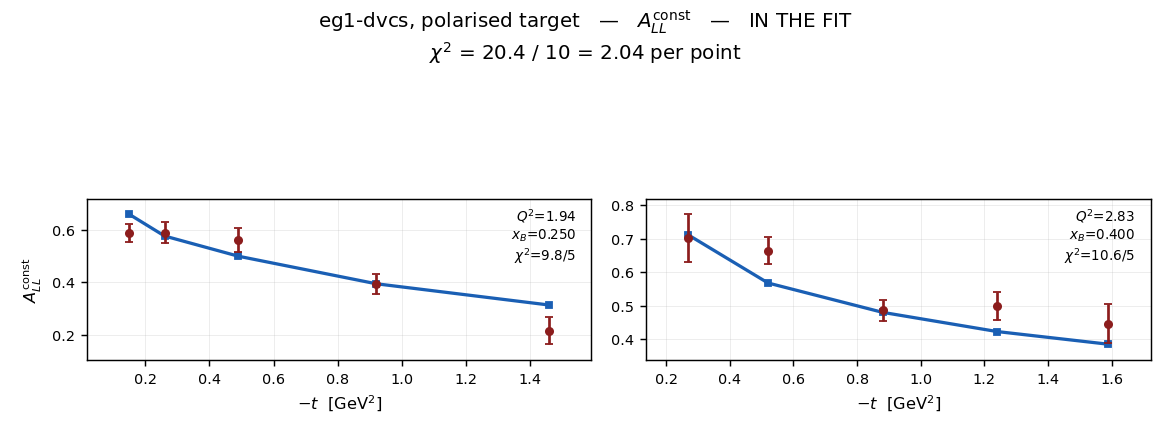
\includegraphics[width=\textwidth]{13_eg1_in_ALLc.png}
\caption{eg1-dvcs, polarised target --- $A_{LL}^{\rm const}$.  This set: $\chi^2 = 71.7/40 = 1.79$ per point.}
\end{figure}

\begin{figure}[p]\centering
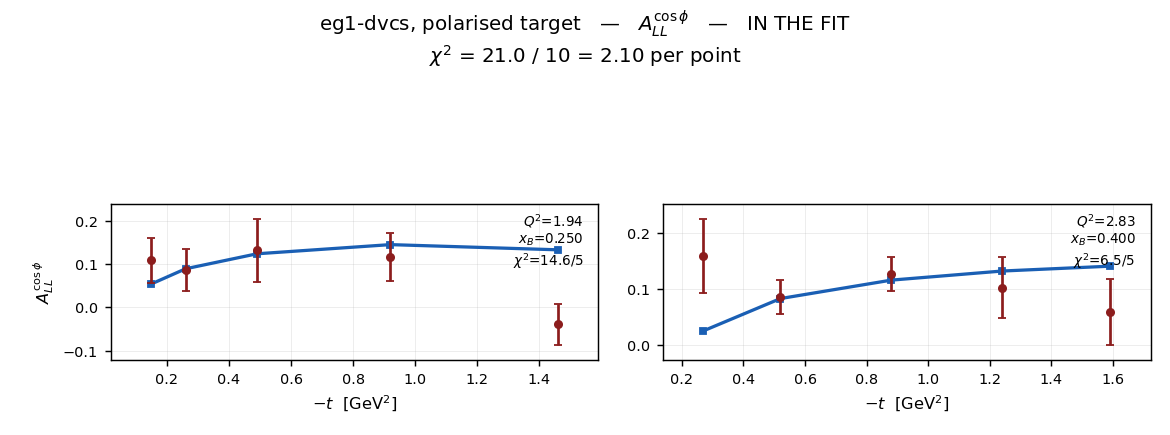
\includegraphics[width=\textwidth]{13_eg1_in_ALLcos.png}
\caption{eg1-dvcs, polarised target --- $A_{LL}^{\cos\phi}$.  This set: $\chi^2 = 71.7/40 = 1.79$ per point.}
\end{figure}

\begin{figure}[p]\centering
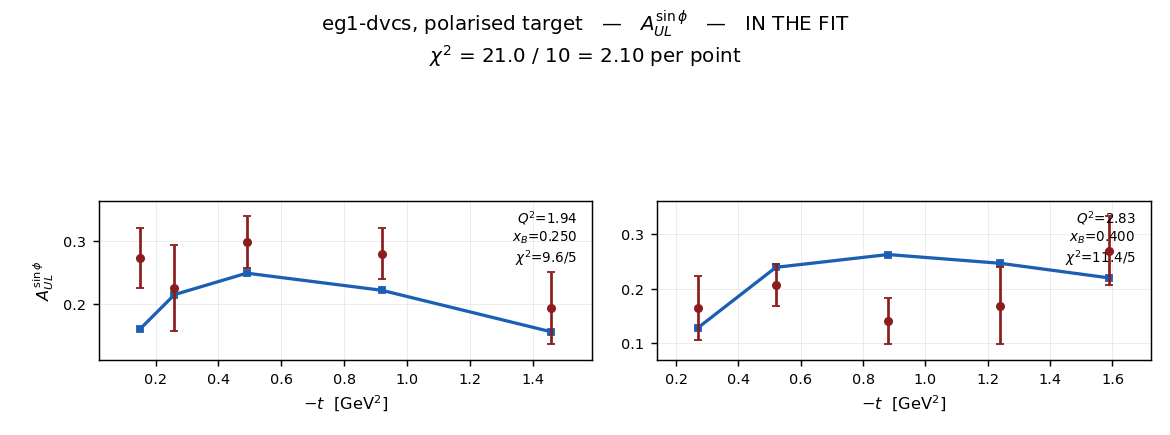
\includegraphics[width=\textwidth]{13_eg1_in_AULsin.png}
\caption{eg1-dvcs, polarised target --- $A_{UL}^{\sin\phi}$.  This set: $\chi^2 = 71.7/40 = 1.79$ per point.}
\end{figure}

\begin{figure}[p]\centering
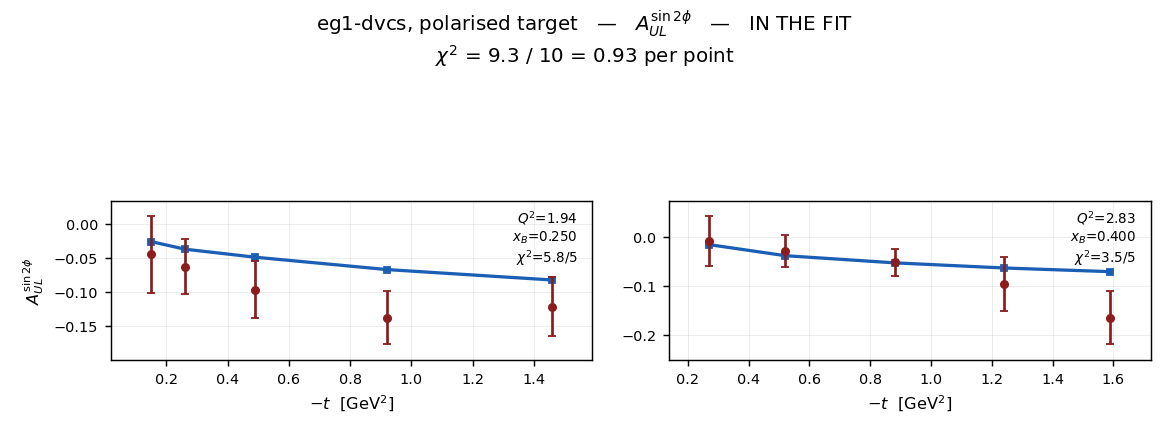
\includegraphics[width=\textwidth]{13_eg1_in_AULsin2.png}
\caption{eg1-dvcs, polarised target --- $A_{UL}^{\sin2\phi}$.  This set: $\chi^2 = 71.7/40 = 1.79$ per point.}
\end{figure}

\end{document}
